\documentclass[11pt]{article}

\usepackage[T1]{fontenc}
\usepackage[margin=1in]{geometry}
\usepackage{amsmath,amssymb,mathtools,amsthm}
\usepackage{booktabs,tabularx,array}
\usepackage{graphicx}
% microtype font expansion requires a scalable T1 font; fall back if lmodern is absent.
\IfFileExists{lmodern.sty}
  {\usepackage{lmodern}\usepackage{microtype}}
  {\usepackage[expansion=false]{microtype}}
\usepackage{enumitem}
\usepackage{tikz}
\usepackage{pgfplots}
\pgfplotsset{compat=1.16}
\usepackage[hidelinks]{hyperref}

\setlength{\parindent}{0pt}
\setlength{\parskip}{0.65em}
\setlist[itemize]{leftmargin=*,itemsep=0.2em,topsep=0.3em}
\setlist[enumerate]{leftmargin=*,itemsep=0.3em,topsep=0.3em}
\renewcommand{\arraystretch}{1.18}
\setcounter{tocdepth}{1}

\newcommand{\AP}{\operatorname{AP}}
\newcommand{\CNAP}{\operatorname{CNAP}}
\newcommand{\Regime}{\mathcal{R}}
\newcommand{\Tpi}{\CNAP_{\pi_\star}}
\newcommand{\E}{\mathbb{E}}
\newcommand{\iid}{\mathrel{\overset{\mathrm{iid}}{\sim}}}

% Supported-performance notation for the average-precision application.
\newcommand{\SAPfull}{S_{2,\pi_\star}^{\mathrm{AP}}(\Regime)}
\newcommand{\SAP}{S_{2,\pi_\star}^{\mathrm{AP}}}
\newcommand{\SAPHat}{\widehat S_{2,\pi_\star}^{\,\mathrm{AP}}}
\newcommand{\SAPHatB}{\widehat S_{2,\pi_\star,B}^{\,\mathrm{AP}}}
\newcommand{\SAPnull}{S_{2,\pi_\star}^{\mathrm{AP,null}}}
\newcommand{\SAPnullHat}{\widehat S_{2,\pi_\star}^{\,\mathrm{AP,null}}}
\newcommand{\SAPcalHat}{\widehat S_{2,\pi_\star}^{\,\mathrm{AP,cal}}}

\newcommand{\PRep}{P_{\mathrm{rep}}^{\Regime,\pi_\star}}
\newcommand{\PRepHat}{\widehat{P}_{\mathrm{rep}}^{\Regime,\pi_\star}}

\newtheorem{definition}{Definition}
\newtheorem{proposition}{Proposition}
\theoremstyle{remark}
\newtheorem*{remark}{Remark}

\title{Supported Predictive Performance\\
\large A Replication-Based Method for Average Precision}
\author{Marcus A. Thomas}
\date{Methodological proposal}

\begin{document}

\maketitle

\begin{abstract}
Predictive performance is usually reported from one evaluation, although its value may vary across replications. For any scalar performance effect $T$ oriented so that larger values are better, define
\[
S_2(T;\Regime)
=
\E_{\Regime}[\min\{T_1,T_2\}],
\]
where $T_1$ and $T_2$ arise from independent executions of a declared evaluation-generating regime $\Regime$. The supported level is the average maximal claim surviving both tests, or expected performance minus half their expected absolute disagreement. More generally, $K$ controls Popperian severity through the number of independent tests a claim must survive.

We develop the method for average precision, whose value and chance level depend on positive-class prevalence. Prior standardization and chance normalization produce a common CNAP scale with population random ranking at zero and perfect ranking at one. Applying the support operator gives a regime-indexed level: the regime declares the mechanisms allowed to vary and the replication size, so the result is not an intrinsic property of the fitted model. A stratified bootstrap represents the canonical fixed-model regime, and conditional-null calibration locates one model relative to its finite-design chance level. Model replacement instead uses paired differences on the uncalibrated CNAP scale. A candidate satisfies the performance-based replacement criterion when its supported advantage exceeds a declared margin $d$; population-level evidence requires an outer lower confidence bound above $d$.
\end{abstract}

\begingroup
\small
\setlength{\parskip}{0pt}
\tableofcontents
\endgroup
\newpage

\section{Comparability and reliability of average-precision evaluations}
\label{sec:problems}

Many prediction systems rank cases so that a selected set can receive further attention, for example, candidate peptides chosen for a vaccine or radiological images assigned for review. In either setting, the evaluation unit receives a score and an outcome, and the model is used by acting on the upper part of the ranked list. Performance must then describe the composition of the selected set as well as separation between the classes.

AUROC describes separation through the probability that a randomly drawn positive outranks a randomly drawn negative. It remains unchanged by positive-class prevalence when the class-conditional score distributions remain fixed. This property does not determine how many selected cases are positive. A small false-positive rate can admit many false positives when negatives are abundant, leaving a high-AUROC model with low selected-set purity. Precision measures that purity, and recall measures the fraction of positives selected. Average precision summarizes both quantities as the threshold is lowered. We use the non-interpolated finite-sample definition
\[
\AP
=
\sum_k (r_k-r_{k-1})p_k,
\]
which assigns each gain in recall the precision at the threshold producing it. Equal scores enter together, and no interpolation is added between observed operating points. Appendix~\ref{app:prevalence} gives the full definition and its relation to other AUPRC conventions.

Cross-dataset comparison becomes difficult because precision depends on population class proportions. At a given threshold, the numbers of selected positives and negatives reflect the class-conditional selection rates applied to the numbers available in each class. Suppose a threshold selects $80\%$ of positives and $5\%$ of negatives. In a balanced population of 10,000 cases, it selects 4,000 positives and 250 negatives, giving precision $0.94$. In a population with $1\%$ positives, the same threshold selects 80 positives and 495 negatives, giving precision $0.14$. The class-conditional selection rates and ranking performance are unchanged. The change in precision arises from the relative numbers of positive and negative cases available for selection. Because AP aggregates precision across thresholds, it inherits this dependence on prevalence. AP values from datasets with different prevalences therefore refer to different target populations.

Comparisons intended to describe the same target population must evaluate selected-set purity at the same prevalence. They also require a common chance level. Population random ranking selects the same fraction of each class, making precision and population AP equal to prevalence. An AP of $0.10$ represents chance performance at prevalence $0.10$ and improvement over chance at prevalence $0.01$. Cross-dataset comparison therefore requires a declared target prevalence and an effect scale with common endpoints for random and perfect ranking.

CNAP supplies a common effect scale, but comparability on that scale still concerns one finite result. Consider two evaluations that each report $0.30$, one with 20 positive cases and the other with 20,000. Each positive changes recall by $0.05$ in the smaller evaluation and by $0.00005$ in the larger one, so a few ranks can move the former much more. The point estimates agree while their behavior across replications can differ because of evaluation size, clustering, ties, influential cases, sites, measurement conditions, or repeated model development.

Supported performance describes corroboration under a declared regime and therefore remains design-indexed. Studies sharing $\pi_\star$ use the same CNAP scale, but their supported values answer the same corroboration question only under compatible regimes, including compatible replication sizes. A prospective comparison can standardize that size. The regime follows the claim: it may hold one fitted model fixed, allow sites to vary, or repeat training, tuning, and selection. AP therefore requires a target prevalence for scale comparability and a regime for corroboration.

\section{Constructing a common average-precision effect scale}
\label{sec:common-scale}

\subsection{Prior-standardized average precision}

Choose a reference prevalence $\pi_\star\in(0,1)$. At score threshold $c$, let
\[
r(c)=\Pr(S\geq c\mid Y=1),
\qquad
f(c)=\Pr(S\geq c\mid Y=0).
\]
These are the true-positive and false-positive rates. Precision in a population with prevalence $\pi_\star$ is
\begin{equation}
 p_{\pi_\star}(c)
 =
 \frac{\pi_\star r(c)}
 {\pi_\star r(c)+(1-\pi_\star)f(c)}.
 \label{eq:main-reference-precision}
\end{equation}

\paragraph{Precision odds separate prevalence from ranking quality.}
Dividing Equation~\eqref{eq:main-reference-precision} by its complement reveals how prevalence and ranking quality enter separately:
\begin{equation}
\underbrace{\frac{p_{\pi_\star}(c)}{1-p_{\pi_\star}(c)}}_{\text{precision odds}}
=
\underbrace{\frac{\pi_\star}{1-\pi_\star}}_{\text{prior odds}}
\times
\underbrace{\frac{r(c)}{f(c)}}_{\text{likelihood ratio}}.
\label{eq:odds}
\end{equation}
Precision odds are a product of two factors. The first depends only on the target population. The second depends only on the class-conditional score distributions and is therefore a property of the ranking model at that threshold. Prevalence enters precision through exactly one factor. The same factorization underlies prior-probability and cost adjustment in classification~\cite{elkan2001foundations}.

Take a threshold selecting $80\%$ of positives and $5\%$ of negatives, so $r=0.8$ and $f=0.05$ and the likelihood ratio is $16$. In a balanced population the prior odds are $1$, precision odds are $16$, and precision is $0.94$. At $1\%$ prevalence the prior odds are $1/99$, precision odds are $16/99$, and precision is $0.14$. The ranking is identical in both. Equation~\eqref{eq:main-reference-precision} replaces the prior-odds factor with a declared value and leaves the likelihood ratio untouched.

Siblini et al.~\cite{siblini2020calibration} use this operation to evaluate precision-based metrics at a fixed reference class ratio. Calibrated average precision in online action detection uses the balanced-reference special case~\cite{degeest2016online}. We adopt the same prior-standardization operation and use $\pi_\star$ for the prevalence of the scientific target population. Section~\ref{sec:related-normalizations} compares this operation with a normalization that removes the prior-odds factor.

Applying Equation~\eqref{eq:main-reference-precision} across all distinct thresholds gives
\[
\AP_{\pi_\star}(D),
\]
the prior-standardized AP of dataset $D$. Appendix~\ref{app:prevalence} gives the finite-sample definition, tie rule, AP convention, and weighted implementation. The stepwise convention used here need not equal a calibrated PR area computed under a different interpolation rule.

The reference prevalence specifies the population in which selected-set purity is interpreted. It should follow the scientific target and remain fixed across evaluations being compared, alongside a common AP convention. Section~\ref{sec:regime} gives the invariance it assumes.

\subsection{Chance normalization}

Prior-standardized AP still has a nonzero random-ranking baseline. For population random ranking, the selected fraction is the same in both classes:
\[
r(c)=f(c).
\]
The likelihood ratio in Equation~\eqref{eq:odds} equals one, so precision odds equal prior odds and
\[
p_{\pi_\star}(c)=\pi_\star.
\]
Population random ranking therefore has prior-standardized AP equal to $\pi_\star$.

Define
\begin{equation}
\Tpi(D)
=
\frac{\AP_{\pi_\star}(D)-\pi_\star}{1-\pi_\star}.
\label{eq:T}
\end{equation}
We call $\Tpi(D)$ chance-normalized average precision at reference prevalence $\pi_\star$. The numerator measures improvement over population random ranking and the denominator is the largest such improvement, so $\Tpi$ is zero for random ranking, one for perfect ranking, and negative below chance. Since $0\leq \AP_{\pi_\star}\leq 1$, its range is $[-\pi_\star/(1-\pi_\star),\,1]$.

Equation~\eqref{eq:T} has the general form
\begin{equation}
\frac{\text{observed}-\text{chance}}{\text{ceiling}-\text{chance}},
\label{eq:kappa-form}
\end{equation}
an affine, kappa-like normalization familiar from chance-corrected agreement statistics~\cite{cohen1960coefficient}. Su, Yuan, and Zhu~\cite{suyuan2015relationship} rescale ordinary AP using the prevalence of the population being evaluated. Bestgen~\cite{bestgen2021fisher} applies the same kappa form using a random-ranking AP baseline under the name chance-corrected AP. Equation~\eqref{eq:T} first standardizes AP to a declared target prevalence $\pi_\star$, which may differ from the observed prevalence, and then uses $\pi_\star$ as the population random-ranking anchor. We have not found this two-stage construction stated explicitly in earlier work. Its role here is to supply the common prevalence-indexed effect scale used by the support functional. We use chance normalization to distinguish this population-scale operation from the conditional-null calibration in Section~\ref{sec:calibration}.

Prior standardization fixes the population and chance normalization fixes the endpoints, so $\Tpi(D)$ is comparable across evaluations sharing $\pi_\star$, AP convention, and target interpretation. It still comes from one finite evaluation.

\subsection{Dependence on the reference prevalence}

Chance normalization preserves the operational dependence on prevalence. At empirical threshold $k$,
\begin{equation}
\frac{p_{\pi_\star,k}-\pi_\star}{1-\pi_\star}
=
\frac{\pi_\star(r_k-f_k)}
{\pi_\star r_k+(1-\pi_\star)f_k}.
\label{eq:threshold-normalized-effect}
\end{equation}
Since the recall increments sum to one,
\begin{equation}
\Tpi(D)
=
\sum_{k=1}^{K}
(r_k-r_{k-1})
\frac{\pi_\star(r_k-f_k)}
{\pi_\star r_k+(1-\pi_\star)f_k}.
\label{eq:T-reference-dependence}
\end{equation}

So $\pi_\star$ sets the value assigned to each recall increment. A smaller reference prevalence weights false positives more heavily, requiring very small false-positive rates to retain a large effect; a larger one credits separation over a broader recall range. In the limit, a threshold with $f_k>0$ contributes nothing as $\pi_\star\to0$, while one with $f_k=0$ and $r_k>0$ contributes one at every $\pi_\star$. Low reference prevalences therefore emphasize the part of the ranking that retrieves positives before any false positive enters.

For $r_k>0$,
\begin{equation}
\lim_{\pi_\star\to1}
\frac{\pi_\star(r_k-f_k)}
{\pi_\star r_k+(1-\pi_\star)f_k}
=
1-\frac{f_k}{r_k}.
\label{eq:precg-limit}
\end{equation}
The right-hand side is one minus the reciprocal of the likelihood ratio in Equation~\eqref{eq:odds}, and Section~\ref{sec:related-normalizations} identifies it as a known prevalence-free quantity. The contribution changes monotonically with $\pi_\star$ whenever its threshold lies entirely on one side of the ROC diagonal:
\begin{equation}
\frac{\partial}{\partial\pi_\star}
\left\{
\frac{\pi_\star(r_k-f_k)}
{\pi_\star r_k+(1-\pi_\star)f_k}
\right\}
=
\frac{f_k(r_k-f_k)}
{\{\pi_\star r_k+(1-\pi_\star)f_k\}^2}.
\label{eq:reference-prevalence-derivative}
\end{equation}
A threshold with $r_k\geq f_k$ has a nondecreasing contribution. A threshold with $r_k<f_k$ has a nonincreasing contribution.

Model ordering can change with $\pi_\star$. A model with a very clean leading segment may win when positives are rare, while one retrieving positives evenly across a wider threshold range wins at a higher reference prevalence. The effect is indexed by the population in which selection is evaluated.

The scientific target should determine $\pi_\star$: the expected prevalence in the population receiving the model for a deployment analysis, one prespecified value for a benchmark. Using each dataset's observed prevalence would restore the comparability problem. When several deployment populations are relevant, report the reference-prevalence profile
\[
\pi_\star
\longmapsto
\Tpi(D)
\]
over a scientifically plausible range, together with one prespecified primary value when the application requires a scalar summary. Appendix Figure~\ref{fig:profile} shows such a profile.

\subsection{Related standardizations and normalizations}
\label{sec:related-normalizations}

Equation~\eqref{eq:odds} isolates prevalence in the prior-odds factor. Precision-recall-gain analysis removes that factor and describes prevalence-free ranking quality~\cite{flach2015prg}; prior standardization instead assigns it the declared value $\pi_\star$ and describes selected-set purity in a target population. The resulting summaries answer different scientific questions. Appendix~\ref{app:precg} gives the threshold-level derivation, explains why their integral summaries do not coincide, and discusses scale coherence. Here, prior standardization and chance normalization retain the population interpretation needed for the common CNAP scale.

\section{Performance across replications}
\label{sec:regime}

A performance claim acquires meaning relative to the conditions under which it could fail. A result for a fixed fitted model may fail when new evaluation units are drawn. A claim about performance at new sites also faces variation among sites. A claim about a development procedure faces variation from training, tuning, and model selection. These claims therefore require different evaluation-generating regimes.

\begin{definition}[Evaluation-generating regime]
A declared evaluation-generating regime $\Regime$ specifies the target conditions under which performance is interpreted, the environments a replication may visit, and the mechanisms assumed invariant across those environments. A replication is one complete execution of $\Regime$. Mechanisms not held invariant are redrawn with the environment.
\end{definition}

The regime determines the sources of failure against which the claim is assessed. The functional $S_2(T;\Regime)$ may be well-defined when the available data do not identify it. An empirical replication procedure generates only the challenges represented by its data and assumptions. Table~\ref{tab:regimes} gives three common regimes.

\begin{table}[ht]
\centering
\caption{Three evaluation-generating regimes. Site variation and model refitting can vary independently.}
\label{tab:regimes}
\begin{tabularx}{\textwidth}{@{}l>{\centering\arraybackslash}X>{\centering\arraybackslash}X>{\centering\arraybackslash}X@{}}
\toprule
& Fixed model & Multi-site & Repeated development \\
\midrule
\emph{Claim is about} & \emph{this fitted model in this population} & \emph{this fitted model in new sites} & \emph{this development procedure} \\
\midrule
Unit sampling & redrawn & redrawn & redrawn \\
Site, batch, calendar period & invariant & redrawn & redrawn \\
Measurement process & invariant & invariant & invariant \\
Replication class counts $n_+^{\mathrm{rep}}$, $n_-^{\mathrm{rep}}$ & declared & declared & declared \\
Fitted model & invariant & invariant & redrawn \\
\bottomrule
\end{tabularx}
\end{table}


Every invariance declaration is a scientific conjecture. Holding the measurement process invariant across a multi-site environment set assumes comparable measurement at sites that may not have been observed. Study design, substantive knowledge, external evidence, and sensitivity analysis can support the assumption. External replication can expose its failure. A failed invariance leaves the estimand attached to a replication that the application does not realize.

Reference prevalence is one component of the regime. It specifies the class prior at which selected-set purity is interpreted and remains fixed across replications. We display $\pi_\star$ separately because it enters AP analytically through the precision-odds factorization. Other components determine which units, environments, measurement conditions, fitted models, and class counts vary. This decomposition permits sensitivity analysis across $\pi_\star$ without changing the resampling mechanism. Equation~\eqref{eq:main-reference-precision} assumes invariant class-conditional score mechanisms. Appendix~\ref{app:prevalence} describes violations caused by changing case mix.

Write $n_+^{\mathrm{obs}}$ and $n_-^{\mathrm{obs}}$ for the observed evaluation counts, and $n_+^{\mathrm{rep}}$ and $n_-^{\mathrm{rep}}$ for the counts generated in a replication. A same-design analysis sets the latter equal to the former. A prospective analysis declares the counts planned for future evaluations. The observed counts govern estimation of the score distributions. The replication counts help define the estimand.

Independence applies to complete replications. It need not hold among observations within a replication. Writing $C$ for the contextual variables allowed to vary, a hierarchical regime draws $C^{(j)}\sim P_{\Regime}(C)$ and then $D^{(j)}\sim P_{\Regime}(D\mid C^{(j)})$. Two evaluations can therefore be independent executions of $\Regime$ while units within a site or measurements within a batch remain dependent.

Two senses of unit must also be distinguished. The evaluation unit receives a score and an outcome. The exchangeable unit is resampled or permuted as a whole. They coincide when evaluation units are independent. Under nesting, the exchangeable unit is the cluster, and the evaluation units inside it move together.

Repeated development requires access to the training data and the complete fitting pipeline. Every replication entails a training run. The conditional-null calibration in Section~\ref{sec:calibration} applies to fixed predictions. A development-level regime can define and estimate $S_2$. Its conditionally calibrated form requires a null construction for the development process.

With $\pi_\star$ and the other components of $\Regime$ declared, independent executions of the regime induce a distribution of chance-normalized AP values.

\subsection{The replication distribution}

Let
\[
D^{\mathrm{rep}}\sim P_{\Regime}
\]
denote one complete execution of $\Regime$, and define
\begin{equation}
\Theta_{\pi_\star}
=
\Tpi(D^{\mathrm{rep}}).
\label{eq:Theta}
\end{equation}

The law of $\Theta_{\pi_\star}$ is the regime-induced replication distribution $\PRep$. Its center describes expected performance across replications at $\pi_\star$. Its shape describes variation across replications. Changing $\pi_\star$ changes this distribution because the dataset generated by each replication is evaluated by a different prevalence-indexed functional.

Replication-based assessment of classifier performance has precedent. Nadeau and Bengio~\cite{nadeau2003inference} study inference for the generalization error across resampled runs, and Bouckaert~\cite{bouckaert2004estimating} studies the replicability of learning experiments. Those treatments target error rate and its variance. The distribution here concerns a prior-standardized, chance-normalized precision effect generated under a declared regime.

An observed evaluation $D_{\mathrm{obs}}$ supplies a data-conditional representation of the regime distribution,
\[
\PRepHat(\,\cdot\mid D_{\mathrm{obs}}).
\]
For the canonical fixed-model implementation, a stratified bootstrap draws $n_+^{\mathrm{rep}}=n_+^{\mathrm{obs}}$ positives and $n_-^{\mathrm{rep}}=n_-^{\mathrm{obs}}$ negatives. It induces a distribution under the observed class-conditional score distributions. Hierarchical simulation, repeated training, and other procedures apply when the regime redraws further mechanisms. The empirical representation limits the evidential scope of the supported value.

\section{The two-replication support operator}
\label{sec:support}

Let $T$ be a performance effect whose larger values indicate better performance. Each level $s$ defines the claim that performance reaches at least $s$. An evaluation yielding $t$ leaves this claim standing when $s\leq t$ and defeats it when $s>t$. The realized effect is the greatest level retained by that evaluation.

Suppose two independent executions of the declared regime produce
\[
t_1=0.70,
\qquad
t_2=0.05.
\]
The first evaluation retains claims through $0.70$. The second retains claims only through $0.05$. A claim made on the strength of both results cannot exceed $0.05$. The larger result supplies no compensation for a level that the second evaluation defeats. This asymmetry is the source of the support criterion.

Formally, a level $s$ is jointly supported when
\[
s\leq t_1,
\qquad
s\leq t_2.
\]
The largest level satisfying these inequalities is
\[
\min\{t_1,t_2\}.
\]
The rule is symmetric, and equal results retain their common value. It expresses corroboration through survival under both evaluations~\cite{popper1959logic}.

For two independent executions of $\Regime$, write
\[
T_1,T_2
\iid
P_{\mathrm{rep}}^{\Regime,T}.
\]
Define
\begin{equation}
S_2(T;\Regime)
=
\E_{\Regime}[\min\{T_1,T_2\}].
\label{eq:support-operator}
\end{equation}
When a replication distribution $P$ is supplied directly, $S_2(T;P)$ denotes the same expectation for independent draws from $P$.

Equation~\eqref{eq:support-operator} averages the greatest retained level over pairs of replications generated by the regime. It remains on the scale of $T$. If $T$ is a chance-normalized performance effect, $S_2$ is expressed in the same units.

When $T$ is bounded below by $L$ and above by $U$,\footnote{Let $M=\min(T_1,T_2)$. For each realized value $m\in[L,U]$, $m=L+\int_L^U\mathbf{1}\{m>s\}\,ds$: the integral is the vertical length from $L$ to $m$, obtained by counting every level $s$ that $m$ exceeds. Taking expectations gives $\E[M]=L+\int_L^U\Pr(M>s)\,ds$. Because $M>s$ exactly when both replications exceed $s$, independence gives $\Pr(M>s)=\Pr(T>s)^2$.}
\begin{equation}
S_2(T;\Regime)
=
L+\int_L^U \Pr_{\Regime}(T>s)^2\,ds .
\label{eq:joint-survival}
\end{equation}
At each effect level $s$, the squared survival probability is the probability that two independent replications both retain the claim. The integral averages that joint survival over the effect scale.

The identity $\min(a,b)=(a+b-|a-b|)/2$ gives
\begin{equation}
S_2(T;\Regime)
=
\E_{\Regime}[T]
-
\frac12\E_{\Regime}[|T_1-T_2|].
\label{eq:general-decomposition}
\end{equation}

$S_2$ equals expected performance across replications minus half the expected disagreement between replications. The second term measures the reduction in the retained claim produced by instability across the regime. No external penalty or sample-size multiplier is introduced.

The result is a supported performance level. It gives no probability that a specified level will recur, that a claim is true, or that a confidence interval covers a parameter. Section~\ref{sec:survival} introduces $m_\gamma$, the level retained by two replications with frequency $\gamma$.

Disagreement between replications lowers the retained level. A regime producing $0.5$ and $0.9$ with equal probability has the same mean as one producing $0.7$ with certainty, and a value of $S_2$ of $0.6$. Whenever either replication returns $0.5$, the pair contributes $0.5$; the value $0.9$ is retained only when both replications attain it. The general statement holds beyond this example: a mean-preserving spread of the replication distribution cannot raise $S_2$. Appendix~\ref{app:properties} obtains this from the concavity of the associated distortion function.

\subsection{Supported chance-normalized average precision}

Set $T=\CNAP_{\pi_\star}$, and let $\Theta_{\pi_\star,1},\Theta_{\pi_\star,2}\iid\PRep$ denote two independent draws from its replication distribution. This specialization gives supported performance for average precision.

\begin{definition}[Supported chance-normalized average precision]
\begin{equation}
\SAPfull
=
S_2(\CNAP_{\pi_\star};\Regime).
\label{eq:rcap}
\end{equation}
\end{definition}

The quantity $\SAPfull$ is a functional of the prevalence-indexed replication distribution. Once the regime is fixed we write $\SAP$. Equation~\eqref{eq:general-decomposition} specializes to
\begin{equation}
\SAP
=
\E_{\Regime}[\Theta_{\pi_\star}]
-
\frac12
\E_{\Regime}
\left[
|\Theta_{\pi_\star,1}-\Theta_{\pi_\star,2}|
\right],
\label{eq:decomposition}
\end{equation}
and changing $\pi_\star$ can move both terms.

\begin{center}
\fbox{\parbox{0.86\linewidth}{
\centering
Supported chance-normalized AP $=$ expected performance across replications $-$ replication-disagreement penalty.
}}
\end{center}

The minimum $M=\min\{\Theta_{\pi_\star,1},\Theta_{\pi_\star,2}\}$ has its own law under the regime. This support distribution records the level two replications jointly retain. Supported chance-normalized AP is its mean, and Section~\ref{sec:survival} describes its lower tail.

Given an observed evaluation, use its empirical replication distribution $\PRepHat(\cdot\mid D_{\mathrm{obs}})$. The resulting data-dependent quantity is
\begin{equation}
\SAPHat
=
S_2(\CNAP_{\pi_\star};\PRepHat)
=
\E_{\PRepHat}
\left[
\min\{
\Theta_{\pi_\star,1},
\Theta_{\pi_\star,2}
\}
\mid D_{\mathrm{obs}}
\right].
\label{eq:rcap-estimated}
\end{equation}

Chance normalization places population random ranking at $\Tpi=0$. A finite-sample chance evaluation can have $\SAP\ne0$. Section~\ref{sec:calibration} measures that level and calibrates the supported value.

\section{Constructing supported performance from one observed evaluation}
\label{sec:estimation}

The population functional $\SAPfull$ belongs to a declared regime. A researcher with one observed evaluation constructs a data-conditional supported value from an empirical replication distribution. Its interpretation remains tied to the mechanisms represented by that construction.

\subsection{Canonical fixed-model estimator}

Suppose $D_{\mathrm{obs}}$ is an independent or held-out evaluation of a fixed fitted model. Let
\[
D_{\mathrm{obs},+}
=
\{(s_i,y_i)\in D_{\mathrm{obs}}:y_i=1\},
\qquad
D_{\mathrm{obs},-}
=
\{(s_i,y_i)\in D_{\mathrm{obs}}:y_i=0\},
\]
with
\[
|D_{\mathrm{obs},+}|=n_+^{\mathrm{obs}},
\qquad
|D_{\mathrm{obs},-}|=n_-^{\mathrm{obs}}.
\]
The canonical estimator sets $n_+^{\mathrm{rep}}=n_+^{\mathrm{obs}}$ and $n_-^{\mathrm{rep}}=n_-^{\mathrm{obs}}$. It uses a stratified bootstrap with $B$ computational replicates. For each bootstrap replicate $b=1,\ldots,B$:
\begin{enumerate}
\item Sample $n_+^{\mathrm{rep}}$ evaluation units with replacement from $D_{\mathrm{obs},+}$.
\item Independently sample $n_-^{\mathrm{rep}}$ evaluation units with replacement from $D_{\mathrm{obs},-}$.
\item Combine the sampled units into $D^{(b)}$. Each bootstrap replicate therefore has the same positive count, negative count, and total size as $D_{\mathrm{obs}}$.
\item Calculate
\[
t_b=\Tpi(D^{(b)})
=
\frac{\AP_{\pi_\star}(D^{(b)})-\pi_\star}{1-\pi_\star}.
\]
\end{enumerate}

Equivalently, if $\widehat P_+$ and $\widehat P_-$ are the empirical distributions of the observed positive and negative evaluation units,
\[
D_+^{(b)}\sim \widehat P_+^{\,n_+^{\mathrm{rep}}},
\qquad
D_-^{(b)}\sim \widehat P_-^{\,n_-^{\mathrm{rep}}},
\qquad
D^{(b)}=D_+^{(b)}\cup D_-^{(b)}.
\]
Bootstrap replicates are generated independently across $b$.

This procedure redraws units and holds every other mechanism invariant. The empirical class-conditional distributions in $D_{\mathrm{obs}}$ approximate the corresponding invariant mechanisms. The resulting replication distribution represents finite-sample variation visible in the observed evaluation, including sensitivity to individual ranks, ties, and the observed class counts. It contains no variation from unobserved sites, instruments, subpopulations, or time periods. The canonical estimator supports a claim within the environment represented by the evaluation. External claims require data or modeling assumptions that span the additional environments.

Prospective replication counts define a different regime and must be stated. Resampling the evaluation set alone is invalid when its outcomes entered training, tuning, or model selection and those stages belong to the claim.

\subsection{Departures from the canonical estimator}

The resampling procedure should change when the declared regime redraws a mechanism the canonical bootstrap holds invariant.

\begin{table}[ht]
\centering
\caption{Departures from the canonical fixed-model bootstrap.}
\label{tab:replication}
\begin{tabularx}{\textwidth}{@{}>{\raggedright\arraybackslash}p{0.34\textwidth}>{\raggedright\arraybackslash}X@{}}
\toprule
Scientific claim & Required departure \\
\midrule
Dependent evaluation units & Resample complete independent units or clusters while preserving their internal dependence. \\
Units nested within fixed clusters & Hold clusters fixed and resample units within each cluster. \\
Clusters recur as a source of variation & Resample or generate clusters under a hierarchical cluster-generating model, then generate units within them. \\
Outcome counts vary across replications & Generate $n_+^{(b)}$ and $n_-^{(b)}$ under the declared prevalence and sampling design. \\
A future evaluation has a different size & Use the declared future positive and negative counts, or their declared distribution, in every generated replicate. \\
Model development recurs & Rerun training, tuning, model selection, and evaluation within each generated replicate. \\
\bottomrule
\end{tabularx}
\end{table}

With very few positive cases, the empirical bootstrap contains little information about unseen positive cases. Parametric score models, Bayesian posterior predictive simulation, sensitivity analysis, or external evaluation may give a more credible estimate of $\PRep$. These procedures still require a declared replication design.

\subsection{Calculate the support functional}

The values $t_1,\ldots,t_B$ are draws from the empirical replication distribution induced by the declared resampling procedure. The all-pairs estimator is
\begin{equation}
\SAPHatB
=
\frac{2}{B(B-1)}
\sum_{1\leq i<j\leq B}
\min(t_i,t_j).
\label{eq:uestimator}
\end{equation}

The equivalent disagreement form is
\begin{equation}
\SAPHatB
=
\bar t
-
\frac{1}{B(B-1)}
\sum_{1\leq i<j\leq B}
|t_i-t_j|.
\label{eq:uestimator-disagreement}
\end{equation}

The calculation uses all distinct pairs. Random pairing adds avoidable Monte Carlo variation. Appendix~\ref{app:computation} gives an $O(B\log B)$ implementation.

The replicate count $B$ controls numerical approximation of the bootstrap functional. The evaluation counts control the information represented in each replicate. Increasing $B$ cannot compensate for a small evaluation. Choose $B$ to make the reported quantity stable at the desired precision, and report its Monte Carlo error. Computationally expensive retraining regimes may require fewer replicates.

\section{Calibrating the conditional chance level}
\label{sec:calibration}

Equation~\eqref{eq:T} assigns zero to population random ranking because $r(c)=f(c)$ implies $\AP_{\pi_\star}=\pi_\star$. The reported supported effect is obtained from resampled finite evaluations. Its chance level need not equal the population value. Two finite-sample effects determine the discrepancy. Their combined contribution must be measured before zero can be interpreted as chance performance.

\subsection{Two finite-sample distortions}

Let $\Regime_0$ be a regime in which the score carries no information about the outcome, and let $\Theta_{\pi_\star}$ be its chance-normalized AP value. Then
\begin{equation}
S_2(\CNAP_{\pi_\star};\Regime_0)
=
\underbrace{\beta(n_+,n_-,\text{ties},\pi_\star)}_{\text{upward bias of }\AP}
\;-\;
\underbrace{\delta(n_+,n_-,\text{ties},\pi_\star)}_{\text{disagreement penalty}} ,
\label{eq:two-distortions}
\end{equation}
where $\beta:=\E[\Theta_{\pi_\star}]$ and $\delta:=\tfrac12\E|\Theta_{\pi_\star,1}-\Theta_{\pi_\star,2}|$.

Both terms are strictly positive in any nondegenerate finite design. Any variability in the replication distribution produces the second term. The first arises because non-interpolated average precision evaluates precision at thresholds selected by the positions of the positive cases themselves. Under random ranking, these positions are favorably placed often enough to lift expected AP above population prevalence. Bestgen~\cite{bestgen2015random} derives the finite-sample expectation of ordinary stepwise AP under uniform random ranking. Manzhos, Ianevych, and Melnyk~\cite{manzhos2026average} give finite-sample moments for AP at a fixed cutoff. Their results establish the general distinction between the population baseline and the finite-evaluation baseline. Conditional permutation accommodates a declared $\pi_\star$, the realized ties, and the complete support procedure.

The residual can be practically visible. Under random ranking with $n=10$, one positive case, and $\pi_\star=0.1$, the supported chance level is $0.0786$: a model with no information earns a positive raw supported score in that finite design. Appendix~\ref{app:null-examples} derives this result, a two-observation example, and the general one-positive formula.

\paragraph{Net finite-sample chance level.}
If the disagreement penalty acted alone, a positive value would be a conservative indication of better-than-chance performance. The AP bias removes that implication. The sign of $\beta-\delta$ depends on the class counts, ties, and $\pi_\star$. The residual is often small in large tie-free evaluations and can be substantial with sparse positives. Conditional permutation measures it for the observed score vector.

\subsection{The conditional fixed-prediction null}
\label{sec:conditional-null}

Suppose a developed prediction rule has been evaluated on independent outcomes that played no role in its development. Let $\mathbf{s}$ be its realized score vector and let $\mathbf{y}$ contain $n_+$ positive and $n_-$ negative outcomes.

\begin{definition}[Conditional fixed-prediction null]
Condition on $\mathbf{s}$, its tie structure, the evaluation units, and the observed class counts. The null distribution assigns outcomes to scores through the permutations allowed by the evaluation design. It imposes exchangeability of outcomes with respect to the fixed scores.
\end{definition}

When the evaluation unit is itself the exchangeable unit, every assignment of $n_+$ positive labels is allowed. Clustered and matched designs make the cluster the exchangeable unit and require restricted permutations that preserve its structure. The score vector remains fixed in every case.

This null challenges the realized predictions. It asks how much supported performance the complete pipeline produces after their association with the outcomes has been removed. The test is conditional on model development. Training, tuning, and model selection have already occurred.

The permutation supplies a conditional no-association test for the fixed predictions~\cite{ojala2010permutation}. A small upper-tail probability shows that few allowed relabellings sustain an effect as large as the observed one.

For each allowed permutation $\sigma$, attach the permuted outcomes $\mathbf{y}^{(\sigma)}$ to $\mathbf{s}$, construct the empirical replication distribution, and apply $S_2$. The conditional chance level is the mean supported effect over this permutation distribution. We write it as $\SAPnull$ once the observed evaluation is understood.

\subsection{Estimating the conditional chance level}

Sample $M$ allowed outcome permutations. For permutation $m$:
\begin{enumerate}
\item Attach the permuted outcomes to the fixed scores.
\item Run the $B$-replicate estimator of Section~\ref{sec:estimation}.
\item Record the resulting supported effect
\[
\widehat S_{2,B}^{(m)}
=
\widehat S_{2,\pi_\star,B}^{\,\mathrm{AP},(m)}.
\]
\end{enumerate}

Estimate the conditional chance level by
\begin{equation}
\SAPnullHat
=
\frac{1}{M}\sum_{m=1}^{M}\widehat S_{2,B}^{(m)}.
\label{eq:conditional-null}
\end{equation}
The upper-tail permutation $p$-value is
\[
p
=
\frac{1+\#\{m:\widehat S_{2,B}^{(m)}\geq\SAPHat\}}{M+1}.
\]

The validity of this test rests on the choice of exchangeable unit. Conditional randomization inference needs no asymptotic reference distribution. Finite $B$ and $M$ add Monte Carlo error, and power can be weak when positive cases are sparse.

The sign of $\SAPnullHat$ shows which finite-sample distortion dominates. A positive value means the upward bias of non-interpolated AP is larger. A negative value means the disagreement penalty is larger.

\subsection{Conditional-null calibration}

The conditional null supplies the lower anchor of the reported scale. The upper anchor is perfect separation, the case in which every positive case outranks every negative case. The canonical estimator attains that anchor exactly.

\begin{proposition}[Perfect-separation fixed point under the canonical bootstrap]
\label{prop:fixed-point}
Suppose every positive score in $D_{\mathrm{obs}}$ exceeds every negative score. Then $t_b=1$ for every stratified bootstrap replicate, so $\PRepHat$ is degenerate at $1$ and $\SAPHat=1$.
\end{proposition}

Appendix~\ref{app:fixed-point-proof} gives the proof.

Proposition~\ref{prop:fixed-point} establishes that the stated upper anchor is attained by the estimator. Without this fixed point, resampling disagreement could make the estimator fall short of one under perfect observed separation. The denominator $1-\SAPnullHat$ would then overstate the attainable range and depress every calibrated value. The fixed point is a property of the canonical bootstrap. Under regimes that rerun training or draw new sites, separation in the observed evaluation need not survive resampling. The calibration developed here is consequently confined to fixed predictions.

\begin{definition}[Conditionally calibrated supported chance-normalized average precision]
\begin{equation}
\SAPcalHat
=
\frac{\SAPHat-\SAPnullHat}{1-\SAPnullHat}.
\label{eq:calibrated}
\end{equation}
\end{definition}

Equation~\eqref{eq:calibrated} requires $\SAPnullHat<1$. It has the form of Equation~\eqref{eq:kappa-form}, with the chance value supplied by the finite-sample conditional null. It places the conditional chance level at zero and perfect separation at one.

\paragraph{Fixed upper anchor.}
A score vector whose ties mix outcomes cannot separate the classes, so no assignment of outcomes to it reaches $\Tpi=1$. For example, a five-level score with $n=200$, $n_+=20$, and $\pi_\star=0.10$ attains at most $0.44$. Normalization by this attainable maximum would remove the shortfall from the reported value. We treat the shortfall as a performance limitation because score resolution is part of the information supplied by a model. A score-specific upper anchor would also change the scale across score representations. Coarsening therefore lowers $\SAPHat$ and $\SAPcalHat$. This treatment charges genuine loss of model resolution and avoidable loss caused by rounding, which motivates the use of unrounded scores in Appendix~\ref{app:prevalence}.

\paragraph{Composition with chance normalization.}
Affine equivariance allows chance normalization to be applied before or after the support operator with the same result; Appendix~\ref{app:affine-equivariance} records the identity.

\paragraph{Reading the calibrated score.}
The calibrated scale is interpreted between its anchors. A supported estimate at or below $\SAPnullHat$ supplies no positive calibrated claim. Such a result is reported as at or below measured chance, with the signed observed effect $\Tpi(D_{\mathrm{obs}})$ giving its direction. Results near the anchor require the permutation $p$-value and the Monte Carlo errors of both supported estimates.

Two models evaluated on the same units rarely share a tie structure. Each has its own $\SAPnullHat$, and Equation~\eqref{eq:calibrated} defines a different affine map for each model. Conditional-null calibration can therefore change their ordering relative to $\SAPHat$. We use calibration to interpret one model relative to its conditional chance level. Paired model comparisons use the common uncalibrated CNAP scale of Section~\ref{sec:paired}. Ordering is preserved when the null levels coincide, as they do for a shared score multiset.

$\SAPcalHat$ is data-conditional because its lower anchor is defined given the realized scores. The regime-indexed functional $\SAPfull$ and the empirical value $\SAPHat=S_2(\CNAP_{\pi_\star};\PRepHat)$ are distinct objects. Identification of the former from the available data requires assumptions connecting $\PRepHat$ to the declared regime. Conditional-null calibration adds a finite-sample permutation reference to the empirical value and does not remove that requirement.

\subsection{Conditions for validity}
\label{sec:caveats}

The permutation distribution represents the sharp null $Y\perp S$ conditional on the realized scores and the permitted outcome assignments. It does not test the weaker statement $\CNAP_{\pi_\star}=0$. A systematically reversed ranker can have $\CNAP_{\pi_\star}<0$ while violating the sharp null.

The permutation holds the scores fixed and moves the outcomes. Its validity requires that no evaluation outcome enter the mechanism producing the scores. A held-out test set satisfies this condition. Ordinary cross-fitting generally does not: a score in one fold depends on outcomes in other folds, so the full outcome vector need not be exchangeable given the full score vector. A cross-fitted analysis requires a permutation design that preserves this dependence, often by rerunning the fitting procedure. The same condition excludes scores from a model whose tuning, feature selection, operating threshold, or stopping rule used the evaluation outcomes. Its assessment requires tracing whether any evaluation outcome reached the scoring mechanism.

A regime that reruns model development can still define and estimate $S_2$. The conditional-null calibration above does not assess that development process. Such a regime needs its own null construction before a calibrated value can be reported.

Appendix~\ref{app:computation} gives the computational cost of the nested permutation and replication procedure.

\subsection{Reporting the sequence of adjustments}
\label{sec:reporting}

Table~\ref{tab:ladder} gives the reporting ladder from the observed evaluation to supported targets and their uncertainty.

\begin{table}[ht]
\centering
\caption{Reporting ladder for observed, replication, and inferential quantities.}
\label{tab:ladder}
\begin{tabularx}{\textwidth}{@{}>{\raggedright\arraybackslash}p{0.22\textwidth}>{\raggedright\arraybackslash}X@{}}
\toprule
Quantity & Question answered \\
\midrule
$\Tpi(D_{\mathrm{obs}})$ & What did this evaluation produce? \\
$\widehat{\E}[\Theta_{\pi_\star}]$ & What is expected under the replication design? \\
$\widehat S_K$ & What average claim survives $K$ replications? \\
$\widehat m_\gamma^{(K)}$ & What claim survives $K$ replications with frequency $\gamma$? \\
Outer interval & How well does this evaluation identify the supported target? \\
\bottomrule
\end{tabularx}
\end{table}

$\SAPcalHat$ is the calibrated headline when the supported effect clears its conditional null. Report $\SAPnullHat$ and the permutation $p$-value with it. The replication mean remains necessary because $\SAPHat$ alone does not identify the mean and disagreement penalty; any two quantities in Equation~\eqref{eq:decomposition} determine the third.

Reports also state $(n_+^{\mathrm{obs}},n_-^{\mathrm{obs}})$, $(n_+^{\mathrm{rep}},n_-^{\mathrm{rep}})$, whether the regime is same-design or prospective, and $K$. Figure~\ref{fig:distribution} relates the replication mean, supported level, and conditional null.

\begin{figure}[ht]
\centering
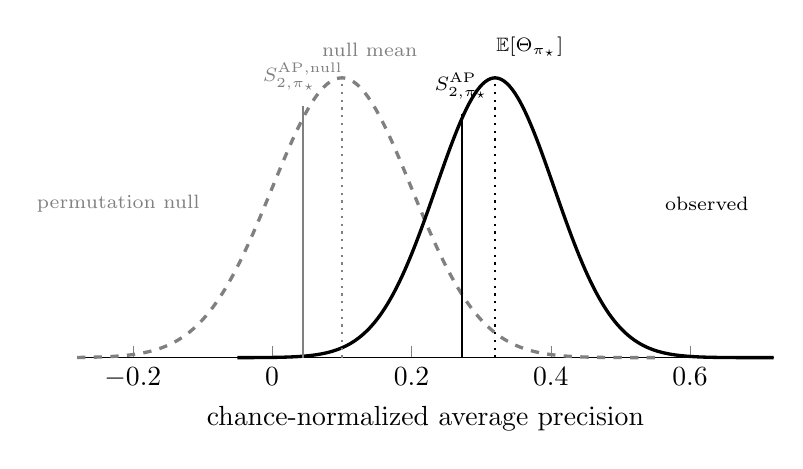
\begin{tikzpicture}
\begin{axis}[
  width=0.86\textwidth, height=6.2cm,
  xlabel={chance-normalized average precision},
  xmin=-0.28, xmax=0.72,
  ymin=0, ymax=1.30,
  axis y line=none,
  axis x line*=bottom,
  xtick={-0.2,0,0.2,0.4,0.6},
  clip=false,
  every axis plot/.append style={very thick},
]
% null replication distribution
\addplot[dashed, gray, domain=-0.28:0.55, samples=200]
  {exp(-((x-0.10)^2)/(2*0.100^2))};
% observed replication distribution
\addplot[solid, black, domain=-0.05:0.72, samples=200]
  {exp(-((x-0.32)^2)/(2*0.085^2))};
% markers
\draw[gray, dotted, thick] (axis cs:0.100,0) -- (axis cs:0.100,1.02);
\draw[gray, thick] (axis cs:0.044,0) -- (axis cs:0.044,0.90);
\draw[black, dotted, thick] (axis cs:0.320,0) -- (axis cs:0.320,1.02);
\draw[black, thick] (axis cs:0.272,0) -- (axis cs:0.272,0.87);
\node[gray, font=\scriptsize, anchor=south] at (axis cs:0.044,0.92) {$\SAPnull$};
\node[gray, font=\scriptsize, anchor=south] at (axis cs:0.14,1.04) {null mean};
\node[font=\scriptsize, anchor=south] at (axis cs:0.272,0.89) {$\SAP$};
\node[font=\scriptsize, anchor=south] at (axis cs:0.37,1.04) {$\E[\Theta_{\pi_\star}]$};
\node[gray, font=\scriptsize, anchor=east] at (axis cs:-0.09,0.55) {permutation null};
\node[font=\scriptsize, anchor=west] at (axis cs:0.55,0.55) {observed};
\end{axis}
\end{tikzpicture}
\caption{Empirical replication distributions for the observed evaluation (solid) and the conditional permutation null (dashed), each summarized by its mean and by $S_2$, which sits below the mean by the disagreement penalty. The null lies above zero, a common result at small positive counts.}
\label{fig:distribution}
\end{figure}

A complete report also states $\pi_\star$, observed and replication counts, the declared regime, resampling and permutation methods, exchangeable units, computational counts, Monte Carlo stability, and how predictions were separated from evaluation outcomes. Appendix~\ref{app:report-example} gives a complete specimen report.

If the supported effect does not clear its conditional null, omit the calibrated headline. Report the result as at or below measured chance, give both supported quantities and the permutation $p$-value, and read direction from the signed observed effect in Equation~\eqref{eq:T}.

When no single target prevalence is scientifically privileged, report
\[
\pi_\star
\longmapsto
\left\{
\Tpi(D_{\mathrm{obs}}),
\SAPHat
\right\}
\]
over a prespecified plausible range, as in Appendix Figure~\ref{fig:profile}. This profile shows whether performance levels, disagreement penalties, or model orderings depend materially on the reference population.

\section{Evaluation size and supported performance}

Evaluation size belongs to the regime. Table~\ref{tab:illustration} considers two prospective designs with the same mean effect and different replication counts. The score distributions and prevalence are held fixed while both class counts scale.

\begin{table}[ht]
\centering
\caption{Illustrative prospective replication distributions with the same mean effect.}
\label{tab:illustration}
\begin{tabular}{@{}lccc@{}}
\toprule
Replication design & $\E[\Theta_{\pi_\star}]$ & $\tfrac12\E|\Theta_{\pi_\star,1}-\Theta_{\pi_\star,2}|$ & $\SAP$ \\
\midrule
$n_+^{\mathrm{rep}}=20$ & $0.30$ & $0.12$ & $0.18$ \\
$n_+^{\mathrm{rep}}=20{,}000$ & $0.30$ & $0.01$ & $0.29$ \\
\bottomrule
\end{tabular}
\end{table}

The smaller design loses more of its mean effect because individual ranks carry greater influence and its replications disagree more. These values are illustrative. Their magnitude depends on both class counts, the score distributions, and ties.

Evaluation size also moves the chance level. The smaller design can have a larger disagreement penalty under permutation and a larger upward AP bias. Conditional-null calibration subtracts their net contribution as measured by the conditional null.

Supported chance-normalized AP contains no multiplicative sample-size factor. The declared replication counts act through the induced replication distribution. If that distribution contracts around a stable value $t_0$,
\[
\SAP\longrightarrow t_0.
\]
Larger evaluations need not produce this contraction under every regime. When they do, the disagreement penalty shrinks while the limiting average-precision scale remains unchanged. Supported values are comparable across studies only under compatible regimes, including compatible replication counts.

\section{Mathematical behavior and interpretive limits}
\label{sec:properties}

\subsection{Basic properties}

A perfectly stable regime incurs no disagreement penalty. If $\Theta_{\pi_\star}=t$ almost surely, then $\SAP=t$. The supported score cannot exceed mean performance across replications and inherits the bounds of its argument. For Equation~\eqref{eq:T}, these bounds are $[-\pi_\star/(1-\pi_\star),\,1]$. First-order stochastic dominance of one replication distribution over another also implies a larger supported value. Appendix~\ref{app:properties} gives proofs, a quantile representation, and connections to two established families of functionals.

The penalty depends on the whole replication distribution. Two distributions sharing a mean and a variance can assign different probability to lower-tail failures and take different supported values.

\subsection{What the reported value does not carry}
\label{sec:collision}

Equation~\eqref{eq:decomposition} combines the center and dispersion of a replication distribution. The resulting scalar does not identify either component by itself. Table~\ref{tab:collision} gives two distributions with the same supported effect.

\begin{table}[ht]
\centering
\caption{Two replication distributions with the same supported effect.}
\label{tab:collision}
\begin{tabular}{@{}lccc@{}}
\toprule
Replication distribution & $\E[\Theta_{\pi_\star}]$ & penalty & $\SAP$ \\
\midrule
$0.9$ and $0.1$ with equal probability & $0.500$ & $0.200$ & $0.300$ \\
$0.3$ with probability one & $0.300$ & $0.000$ & $0.300$ \\
\bottomrule
\end{tabular}
\end{table}

The first design alternates between a strong result and a weak one. The second returns the same intermediate value in every replication. Their supported effects agree despite their different replication behavior.

Section~\ref{sec:reporting} requires $\widehat{\E}[\Theta_{\pi_\star}]$ for this reason. Equation~\eqref{eq:decomposition} is an identity, so any two of its three quantities fix the third. Read as mean and penalty, the first design is $(0.500,0.200)$ and the second $(0.300,0.000)$.

The mean and disagreement penalty still do not determine the lower tail. Appendix~\ref{app:collision-tail} gives two distributions agreeing on both quantities and on $\SAP$ but differing in $m_{0.5}$. Section~\ref{sec:survival} therefore adds $m_\gamma$ whenever a decision depends on a frequency-qualified lower tail.

\subsection{Relation to a standard-error adjustment}

For a replication distribution that is approximately normal with standard deviation $\sigma$, $\E|\Theta_1-\Theta_2|=2\sigma/\sqrt{\pi}$, so
\begin{equation}
\SAP
\approx
\E[\Theta_{\pi_\star}]-\frac{\sigma}{\sqrt{\pi}}
\approx
\E[\Theta_{\pi_\star}]-0.564\,\sigma .
\label{eq:se-approximation}
\end{equation}
Here $\pi$ in the denominator is the circle constant. Under normality, $S_2$ equals the mean shifted down by $0.564$ replication standard deviations. It lies at approximately the $29$th percentile of that distribution. This may resemble a one-sided $71.4\%$ lower bound in the canonical bootstrap.

$S_2$ averages joint survival under the declared regime. A confidence bound addresses uncertainty in estimating a parameter. Outer inference remains necessary when a conclusion depends on the sign of $S_2$. The normal constant can misstate the penalty for skewed or discrete replication distributions. Sparse positives and heavy ties often produce those shapes. The exact minimum form requires only a finite first moment.

The supported score and an uncertainty interval answer different questions. Section~\ref{sec:reporting} gives the estimate, and Section~\ref{sec:error} gives its uncertainty.

\subsection{Monte Carlo error and estimation error}
\label{sec:error}

$\SAPHatB$ has Monte Carlo error from finite $B$. Its interpretation as an estimate of $\SAPfull$ also depends on the sampling assumptions that connect the empirical replication procedure to $\PRep$.

Equation~\eqref{eq:uestimator} is a U-statistic of degree two. Appendix~\ref{app:mcse} gives its Hoeffding-projection estimate of Monte Carlo error, which falls at rate $B^{-1/2}$~\cite{hoeffding1948ustat}.

Increasing $B$ leaves estimation error unchanged. That error is governed by the evaluation units and their class counts. A nested bootstrap measures it by resampling evaluation units in an outer loop and running the complete estimator within each outer dataset. Influence-function methods for L-moments give an analytic alternative when their large-sample approximation is credible~\cite{hosking1990lmoments}. Section~\ref{sec:superiority} uses this outer loop to bound supported superiority in a paired comparison.

The calibrated score also contains Monte Carlo error from estimating $\SAPnullHat$. A delta-method calculation may use independent random streams for $\SAPHat$ and $\SAPnullHat$. Shared random numbers require their covariance. Report the first-order Monte Carlo errors routinely. A conclusion that turns on the distance from the conditional null should also report the nested-bootstrap spread.

\subsection{The support distribution and a survival level}
\label{sec:survival}

The support distribution has a simple form. Let $F$ be the distribution function of $\Theta_{\pi_\star}$ and $Q_{\pi_\star}$ its quantile function. Two independent replications give
\[
\Pr(M>m)=\{1-F(m)\}^2,
\qquad
M=\min\{\Theta_{\pi_\star,1},\Theta_{\pi_\star,2}\}.
\]
The level retained by both replications with frequency $\gamma$ is
\begin{equation}
m_\gamma=Q_{\pi_\star}(1-\sqrt{\gamma}).
\label{eq:survival-level}
\end{equation}
$\SAP$ is the mean of $M$, and $m_\gamma$ is a quantile of the same distribution. Under approximate normality, $\SAP$ lies near $m_{0.5}$. This is a distribution-specific numerical relation and gives $\SAP$ no fixed frequency interpretation. The summaries separate for lumpy distributions. If $\Theta_{\pi_\star}=1$ with probability $0.9$ and $0$ otherwise, $\SAP=0.81$ and $m_{0.9}=0$. The gap shows how an average retained level can coexist with frequent lower-tail failure.

The empirical estimate is an order statistic of the replication array, given in Appendix~\ref{app:survival-computation}. It has the same data-conditional status as $\SAPHat$ and is not a confidence bound for a population parameter. A tail quantile is noisier than the mean and needs a larger $B$. For general $K$, $m_\gamma^{(K)}=Q_{\pi_\star}(1-\gamma^{1/K})$. The choices of $K$ and reporting frequency $\gamma$ remain distinct.

\subsection{Random ranking and the calibrated zero}

The chance-normalized effect $\Tpi$ places population random ranking at zero, and the support functional retains the finite-sample residual of Equation~\eqref{eq:two-distortions}. For fixed predictions, Equation~\eqref{eq:conditional-null} measures that residual and Equation~\eqref{eq:calibrated} removes it.

The signed score preserves below-chance information. Clipping at zero changes finite-sample behavior near chance and should be avoided.

\subsection{Dependence on the reference prevalence}

Changing $\pi_\star$ changes the effect assigned to the dataset generated by each replication and with it the center, shape, and lower tail of the replication distribution. A low reference prevalence makes early false positives especially influential, and the resulting effect on disagreement depends on the score distributions, class counts, ties, and dependence structure. The permutation null must be recomputed at each $\pi_\star$ for which a calibrated value is reported. Since model rankings can reverse across $\pi_\star$, a claim of greater supported performance should state the reference prevalence or the range over which the ordering holds.

\subsection{Dependence on the declared regime}

$\SAP$ is conditional on the declaration of Section~\ref{sec:regime}. Widening the environment set or releasing a mechanism changes the question being answered. Sensitivity analysis can compare plausible declarations, and external replication tests whether the stated invariances survive changes in site, time, instrument, or population composition. A value carries external meaning only when the declared environment set spans the changes at issue.

\subsection{Sparse positive cases}
\label{sec:sparse}

Small positive counts make AP discrete and sensitive to individual ranks. They also limit empirical estimation of the positive score distribution, and they inflate both terms in Equation~\eqref{eq:two-distortions}. A low supported value can reflect weak performance across replications, broad variation across replications, limited information for constructing $\PRepHat$, or a combination of these features. Reporting $\SAPnullHat$ shows what the same pipeline retains after the observed association has been removed. Its tail rests on the same small positive count, so the benchmark is least reliable where the supported level is hardest to estimate.

\subsection{Replication count and Popperian severity}

The parameter $K$ controls Popperian severity by specifying the number of independent tests a performance claim must survive~\cite{popper1959logic}. Severity here means exposure to potentially falsifying tests; it does not denote Mayo's error-statistical severity or carry an error-probability interpretation~\cite{mayo1996error}. The regime determines how demanding each test is, so $K$ is a severity parameter within a declared regime rather than a complete measure of test severity. Define
\[
S_K
=
\E\left[
\min(\Theta_{\pi_\star,1},\ldots,\Theta_{\pi_\star,K})
\right],
\]
and, for effects bounded by $L$ and one,
\[
S_K
=
L+\int_L^1\Pr(\Theta_{\pi_\star}>s)^K\,ds .
\]
The integrand is the probability that all $K$ replications retain level $s$. Increasing $K$ lowers $S_K$ for any nondegenerate distribution and applies a stricter criterion within the fixed regime. Appendix~\ref{app:properties} gives the corresponding quantile weight.

The limit as $K\to\infty$ is the essential infimum of $\Theta_{\pi_\star}$. A finite sample cannot estimate this strict criterion reliably because the estimate reduces to its worst available replicate. The default $K=2$ is the smallest replication count that can test joint survival. Larger values state stricter criteria and are declared with the regime.

\subsection{Centering}

Equation~\eqref{eq:rcap} is replication-centered. A data-centered alternative preserves the observed point estimate and subtracts the estimated penalty. Appendix~\ref{app:centering} states both forms. Simulation must assess their finite-sample behavior. The replication-centered form remains the primary estimand because both terms refer to the same regime distribution.

\section{Paired comparisons and other performance effects}
\label{sec:paired}

\subsection{Paired model comparison}

Support for one model does not determine support for its advantage over another. The comparison must be formed within each replication so that shared changes in evaluation difficulty remain paired. Suppose models $A$ and $B$ are evaluated on the same execution $D^{\mathrm{rep}}$ of the declared regime. Their comparative performance is
\begin{equation}
\Delta_{\pi_\star}
=
\CNAP_{A,\pi_\star}(D^{\mathrm{rep}})
-
\CNAP_{B,\pi_\star}(D^{\mathrm{rep}}).
\label{eq:paired-difference}
\end{equation}
A positive value favors model $A$, a negative value favors model $B$, and zero represents equal chance-normalized average precision at reference prevalence $\pi_\star$. Datasets generated by replications that are easy or difficult for both models can then contribute little variation to the paired difference.

Two independent executions of the regime produce
\[
\Delta_{\pi_\star,1},
\Delta_{\pi_\star,2}
\iid
P_{\mathrm{rep}}^{\Regime,\Delta_{\pi_\star}}.
\]
A superiority level $s$ is retained by both replications when
\[
s\leq \Delta_{\pi_\star,1},
\qquad
s\leq \Delta_{\pi_\star,2}.
\]
The largest such level is their minimum. Define supported superiority by
\begin{equation}
S_2(\Delta_{\pi_\star};\Regime)
=
\E_{\Regime}
\left[
\min\{
\Delta_{\pi_\star,1},
\Delta_{\pi_\star,2}
\}
\right].
\label{eq:paired}
\end{equation}
Using the minimum identity gives
\begin{equation}
S_2(\Delta_{\pi_\star};\Regime)
=
\E_{\Regime}[\Delta_{\pi_\star}]
-
\frac12
\E_{\Regime}
\left[
|\Delta_{\pi_\star,1}-\Delta_{\pi_\star,2}|
\right].
\label{eq:paired-decomposition}
\end{equation}
The first term is the expected advantage of model $A$ across replications. The second term is half the expected disagreement between advantages observed in independent replications. A positive value retains a positive advantage for model $A$ under the two-replication criterion. A nonpositive value supplies no positive supported-superiority claim for model $A$.

For estimation, evaluate both models on every resampled dataset $D^{(b)}$. Define
\[
t_{A,b}=\CNAP_{A,\pi_\star}(D^{(b)}),
\qquad
t_{B,b}=\CNAP_{B,\pi_\star}(D^{(b)}),
\qquad
\delta_b=t_{A,b}-t_{B,b}.
\]
The same resampled evaluation units and outcomes are used for both models within replicate $b$. This preserves the pairing and allows shared changes in evaluation difficulty to cancel in $\delta_b$. The all-pairs estimator is
\begin{equation}
\widehat S_{2,B}(\Delta_{\pi_\star};\Regime)
=
\frac{2}{B(B-1)}
\sum_{1\leq i<j\leq B}
\min(\delta_i,\delta_j).
\label{eq:paired-estimator}
\end{equation}

Identical rankings give $\delta_b=0$ in every replicate. Models with different score structures can retain a nonzero supported difference under joint no-signal outcomes, because their finite-sample AP biases differ.

\subsection{Replacement criterion and inference}
\label{sec:superiority}

Conditional-null calibration of a single model uses the sharp null $Y\perp S$. It states that the realized scores carry no outcome information, and permutation generates its conditional reference distribution.

Model equality has no corresponding sharp permutation null. Both models may carry signal, and their score structures need not be exchangeable. Superiority inference therefore targets the paired estimand directly.

Let $d\geq0$ denote the smallest retained advantage that would justify replacing model $B$ with model $A$. The replacement criterion is
\[
S_2(\Delta_{\pi_\star};\Regime)>d .
\]
The choice $d=0$ requires a positive retained advantage. A positive margin expresses a practical replacement threshold.

Under equal mean performance,
\[
S_2(\Delta_{\pi_\star};\Regime)
=
-\tfrac12\E_{\Regime}\left[|\Delta_{\pi_\star,1}-\Delta_{\pi_\star,2}|\right]
<
0
\]
for a nondegenerate replication distribution. The boundary for margin $d$ is
\[
\E_{\Regime}[\Delta_{\pi_\star}]
=
d+\tfrac12
\E_{\Regime}\left[|\Delta_{\pi_\star,1}-\Delta_{\pi_\star,2}|\right],
\]
so the mean advantage must exceed the practical margin plus half the expected disagreement between replications.

The point estimate reports supported superiority under the empirical regime. Population-level evidence for replacement requires an outer lower confidence bound above $d$. The Monte Carlo standard error in Equation~\eqref{eq:mcse} measures only the accuracy of the inner all-pairs average at fixed $\PRepHat$.

The outer procedure of Section~\ref{sec:error} resamples evaluation units and measures how well one evaluation identifies the support functional. Report its interval whenever a conclusion depends on crossing $d$.

The disagreement penalty can skew the estimator, and the minimum kernel is nondifferentiable at equal arguments. Sparse positive counts and heavy ties increase discreteness near zero. Studentized or bias-corrected intervals may improve on percentile intervals. Their coverage requires simulation.

The replacement claim is relative to the declared regime. Contraction around a stable center raises $S_2(\Delta_{\pi_\star};\Regime)$ toward its mean and may tighten the interval. The result must state the regime, reference prevalence, margin $d$, and outer interval.


\subsection{Marginal values cannot be differenced}

Subtracting two marginal supported values gives a different quantity, and the direction of the discrepancy is fixed.

\begin{proposition}[Marginals overstate supported superiority]
Let $\CNAP_{A,\pi_\star}$ and $\CNAP_{B,\pi_\star}$ have finite first moments under $\Regime$, with any joint law. Then
\[
S_2(\CNAP_{A,\pi_\star};\Regime)
-
S_2(\CNAP_{B,\pi_\star};\Regime)
\;\geq\;
S_2(\Delta_{\pi_\star};\Regime),
\]
with equality if and only if $\CNAP_{B,\pi_\star}$ and $\Delta_{\pi_\star}$ are comonotone.
\end{proposition}

Appendix~\ref{app:marginal-proof} gives the proof and a numerical example. Differencing marginals therefore never understates model $A$'s supported advantage. It compares separate replication summaries rather than applying the criterion to within-replication differences. Marginal supported values from separate studies cannot establish supported superiority; the comparison requires common paired replications.

\subsection{Scope beyond average precision}

The population operator in Equation~\eqref{eq:support-operator} applies to any scalar effect oriented so that larger values indicate better performance. Examples include AUROC, correlation, $R^2$, subgroup contrasts, and paired improvements. For a loss $L(D)$, use $T(D)=-L(D)$. For comparison of two models by loss, use
\[
T(D)=L_B(D)-L_A(D),
\]
so positive values favor model $A$.

Each application requires a replication regime and estimator suited to its scientific claim. A calibrated score further requires metric-specific chance and upper anchors and a valid null construction. This paper develops these elements for AP under the fixed-model regime. Contrasts between models or subgroups follow Section~\ref{sec:superiority}. A positive estimate reports estimated support for the contrast. Formal population-level inference can use a lower confidence bound above zero. The performance effect and study design determine these choices.

\section{Empirical illustration: supported performance in Bank Marketing}
\label{sec:bank-marketing}

\subsection{Data, models, and evaluation regimes}

The Bank Marketing data contain 41,188 telephone marketing contacts ordered by date, with subscription to a term deposit as the positive outcome~\cite{moro2014bank}. The first 80\% of records, $n=32{,}950$, formed the training set. The remaining $8{,}238$ records formed a temporal holdout containing 2,540 positive outcomes. The training prevalence was $0.06373$, and the holdout prevalence was $0.3083$. The training prevalence supplied the primary reference prevalence $\pi_\star$ so that selected-set purity retained the interpretation of the population used to fit the models.

Three fixed model specifications were fitted. A full logistic regression and a random forest used all available pre-contact features. A demographic logistic regression used age, job, marital status, and education. Categorical variables were represented by one-hot indicators. Call duration was excluded because its value is known only after the contact whose outcome is being predicted. Every reported score came from the temporal holdout.

The fixed-model regime held each fitted model fixed and resampled evaluation units within outcome class. This stratified bootstrap preserved the observed positive and negative counts in each empirical replication. Conditional-null calculations held the score vector fixed and permuted outcomes. Paired comparisons used the same resampled rows and outcomes for both models within each replication. These choices target the reproducibility of the fitted models' evaluation under the empirical class-conditional score distributions.

\subsection{Prevalence transport and the common effect scale}

The full logistic model supplied one pair of empirical class-conditional score pools. Samples drawn from those pools had prevalences from $0.02$ to $0.40$. The fitted model and the score distributions conditional on outcome remained fixed. Traditional AP rose from $0.069$ at $2\%$ prevalence to $0.626$ at $40\%$ prevalence, as shown in Figure~\ref{fig:bank-prevalence}. The change follows from the number of negative cases available to enter selected sets.

Prior-standardized AP,
\[
\AP_{\pi_\star}(D),
\]
evaluated every sample at $\pi_\star=0.06373$. Its corresponding values were $0.180$ and $0.158$. The small residual movement reflects sampling variation in the empirical class-conditional score distributions. Chance normalization then gives
\[
\Tpi(D)
=
\frac{\AP_{\pi_\star}(D)-\pi_\star}{1-\pi_\star},
\]
the common effect scale used by the support functional. The reference prevalence determines the population in which precision is read, while chance normalization fixes random ranking at zero and perfect ranking at one.

\begin{figure}[htbp]
\centering
\includegraphics[width=\textwidth]{manuscript_images/01-prevalence-transport.pdf}
\caption{Prevalence transport for the full logistic regression. Each point is the mean over 30 samples from the same held-out class-conditional score pools; bands are the 10th and 90th percentiles. Traditional AP inherits the prevalence of each evaluation sample. Prior-standardized AP evaluates every sample at $\pi_\star=0.06373$. The dotted line marks that primary reference prevalence.}
\label{fig:bank-prevalence}
\end{figure}

\subsection{Observed performance and supported performance}

Two samples of 120 held-out logistic-regression predictions, each containing eight positive outcomes, were selected to have nearly equal observed effects and replication means. Their observed chance-normalized AP values were $0.254$. Their bootstrap means were $0.311$ and $0.308$. Panel A of Figure~\ref{fig:bank-matched-support} therefore gives the same point-performance account for both samples.

Panel B displays their empirical replication distributions. The circles mark
\[
\widehat{\E}[\Theta_{\pi_\star}],
\]
and the diamonds mark
\[
\SAPHat
=
\widehat{\E}[\Theta_{\pi_\star}]
-
\frac12
\widehat{\E}
\left[
\left|
\Theta_{\pi_\star,1}-\Theta_{\pi_\star,2}
\right|
\right].
\]
The more reproducible sample had $\SAPHat=0.249$ and a disagreement penalty of $0.061$. The less reproducible sample had $\SAPHat=0.216$ and a disagreement penalty of $0.092$. Supported chance-normalized AP separates replication distributions that their observed effects and means leave nearly indistinguishable. The samples were selected for this comparison, so their contrast illustrates the support functional and does not estimate a population frequency.

\begin{figure}[htbp]
\centering
\includegraphics[width=\textwidth]{manuscript_images/02-same-performance-different-support.pdf}
\caption{Matched real-data evaluations from the full logistic model. Panel A reports $\Tpi(D_{\mathrm{obs}})$ for two held-out samples with $n=120$ and eight positive outcomes. Panel B shows their canonical bootstrap distributions based on $B=5{,}000$ replications. Circles mark $\widehat{\E}[\Theta_{\pi_\star}]$; diamonds mark $\SAPHat$. The vertical distance between them is the empirical replication-disagreement penalty.}
\label{fig:bank-matched-support}
\end{figure}

\subsection{Conditional chance and calibration}

Population random ranking has $\CNAP_{\pi_\star}=0$, but the supported chance level varied materially with positive count and score resolution. At five positive outcomes, $\SAPnullHat$ ranged from $0.004$ for two score levels to $0.045$ for continuous scores; at 100 positives, it ranged from $-0.001$ to $0.003$. Conditional-null calibration then restored the mean null value to approximately zero across four real-score designs: means before calibration ranged from $-0.001$ to $0.024$, compared with $-0.001$ to $0.000$ afterward. Appendix~\ref{app:bank-diagnostics} gives the design grid, calibration distributions, and computational details. These diagnostics support the use of a design-specific lower anchor; population-level interval performance still requires simulation.

\subsection{Sparse positive outcomes}

The sparse-outcome experiment varied the positive count from 5 to 100 at prevalence near $\pi_\star$. The median complete adjustment, $\Tpi(D_{\mathrm{obs}})-\SAPcalHat$, declined from $0.050$ to $0.008$, while its 10th to 90th percentile interval narrowed from $0.038$--$0.091$ to $0.006$--$0.012$. The adjustment was therefore largest where positive information was scarcest. Appendix~\ref{app:bank-diagnostics} displays the full reporting sequence and profile. This tendency is not guaranteed under every score distribution, tie pattern, or sampling design.

\subsection{Supported model replacement}

For candidate model $A$ and baseline model $B$, the observed paired effect is
\[
\Delta_{\pi_\star}(D_{\mathrm{obs}})
=
\CNAP_{A,\pi_\star}(D_{\mathrm{obs}})
-
\CNAP_{B,\pi_\star}(D_{\mathrm{obs}}).
\]
Applying the support functional to the paired bootstrap differences gives
\[
\widehat S_{2,B}
(\Delta_{\pi_\star};\Regime),
\]
the estimated supported superiority of model $A$.

Figure~\ref{fig:bank-superiority} compares two replacement questions. The random forest exceeded the full logistic model by an observed $0.0034$ on the CNAP scale. Supported superiority was $0.0014$, retaining 41\% of the observed advantage. The full logistic model exceeded the demographic logistic model by $0.0769$, with supported superiority of $0.0741$, retaining 96\%. The demographic model serves as a positive control for a substantial difference.

Each full bar represents $\Delta_{\pi_\star}(D_{\mathrm{obs}})$, and its colored portion represents $\widehat S_{2,B}(\Delta_{\pi_\star};\Regime)$. The gray portion is the total observed-to-supported adjustment:
\[
\Delta_{\mathrm{obs}}-\widehat S_2(\Delta)
=
\left\{
\Delta_{\mathrm{obs}}-\widehat{\E}[\Delta]
\right\}
+
\left\{
\widehat{\E}[\Delta]-\widehat S_2(\Delta)
\right\}.
\]
The second term is the replication-disagreement penalty in Equation~\eqref{eq:paired-decomposition}. The first term is the difference between the observed advantage and its empirical replication mean.

\begin{figure}[htbp]
\centering
\includegraphics[width=\textwidth]{manuscript_images/06-supported-model-superiority.pdf}
\caption{Observed advantage and supported superiority on the Bank Marketing temporal holdout at $\pi_\star=0.06373$. Each full bar is $\Delta_{\pi_\star}(D_{\mathrm{obs}})$. The colored portion is $\widehat S_{2,B}(\Delta_{\pi_\star};\Regime)$ from $B=3{,}000$ paired bootstrap replications. The remaining portion is the total observed-to-supported adjustment. Both models use the same evaluation rows within every paired replication.}
\label{fig:bank-superiority}
\end{figure}

The same-design profile in Appendix~\ref{app:bank-diagnostics} varies both observed information and the replication counts inherited by the canonical bootstrap. With five positive outcomes, median observed and supported differences were $-0.0049$ and $-0.0285$; with 100, they were $0.0037$ and $-0.0014$. These rows answer different corroboration questions and do not estimate one fixed prospective target. A prospective profile must instead hold the target replication design fixed while observed information varies.

\subsection{Reference prevalence and the target population}

The paired model comparison is indexed by the reference prevalence:
\[
\pi_\star
\longmapsto
\left\{
\Delta_{\pi_\star}(D_{\mathrm{obs}}),
\widehat S_2(\Delta_{\pi_\star};\Regime)
\right\}.
\]
Figure~\ref{fig:bank-superiority-prevalence} holds both fitted models, the temporal holdout rows, and the paired bootstrap resamples fixed while $\pi_\star$ ranges from $0.01$ to $0.50$. The blue curve gives the observed target-standardized difference. The orange curve gives supported superiority. The shaded region is their observed-to-supported adjustment.

The observed random-forest advantage remained positive over the plotted range. Supported superiority was positive over the sampled grid from approximately $0.014$ to $0.212$. At the primary reference prevalence of $0.06373$, the observed advantage was $0.0034$ and supported superiority was $0.0014$. At a reference prevalence of $0.50$, the corresponding values were $0.0010$ and $-0.0032$. The fitted models can therefore retain the same observed ordering while the support for a replacement claim changes with the target population.

The profile treats prevalence as the population change and holds the class-conditional score distributions invariant, as required by Equation~\eqref{eq:main-reference-precision}. Covariate shift or concept shift can change those distributions and requires a regime that represents the additional variation.

\begin{figure}[htbp]
\centering
\includegraphics[width=\textwidth]{manuscript_images/08-target-prevalence-model-superiority.pdf}
\caption{Reference-prevalence profile for random forest minus full logistic regression. The observed curve is $\Delta_{\pi_\star}(D_{\mathrm{obs}})$, and the supported curve is $\widehat S_{2,B}(\Delta_{\pi_\star};\Regime)$. One paired sweep with $B=3{,}000$ shared bootstrap replications evaluates all reference prevalences. The vertical dotted line marks the primary value $\pi_\star=0.06373$. The interpretation assumes invariant class-conditional score distributions across target prevalences.}
\label{fig:bank-superiority-prevalence}
\end{figure}

\clearpage

\section{Conclusion}

Predictive-performance reporting supports two tasks. One is to interpret the evidence for a model considered on its own. The other is to inform a choice between models when they can be evaluated together. Both tasks use the same performance scale and replication framework. Each calls for a summary matched to its evidential purpose.

For average precision, reference prevalence $\pi_\star$ gives selected-set purity a common target-population interpretation. Chance normalization places population random ranking at zero and perfect ranking at one. The support operator then measures the performance level retained across independent executions of a declared regime. For any effect $T$ oriented so that larger values are better and $K$ independent executions of the regime,
\[
S_K(T;\Regime)
=
\E_{\Regime}\left[\min(T_1,\ldots,T_K)\right].
\]
This is the average maximal performance claim that survives all $K$ executions. At the default $K=2$, it has the decomposition
\[
S_2(T;\Regime)
=
\E_{\Regime}[T]
-\frac12\E_{\Regime}|T_1-T_2|
\;.
\]
The first term is expected performance across replications. The second is half the expected disagreement between two replications. Increasing $K$ requires a claim to survive more independent replications and gives a more severe criterion within the same regime. Every supported value remains indexed to that regime, which declares the environments, mechanisms, and replication counts allowed to vary.

For a fixed model evaluated on held-out outcomes, the canonical stratified bootstrap estimates the replication distribution under the observed class-conditional score distributions. Finite-sample chance effects remain after population chance normalization. Permuting outcomes against fixed scores measures these effects while preserving the observed class counts and tie structure. The calibrated score
\[
\SAPcalHat
=
\frac{\SAPHat-\SAPnullHat}{1-\SAPnullHat}
\]
assigns the conditional chance level zero and perfect separation one. It describes how much performance a model retains relative to the chance level of its finite evaluation design. This single-model interpretation is especially useful when joint predictions from competing models are unavailable.

Separately reported calibrated supported values can permit cautious benchmarking. Meaningful benchmarking requires a common reference prevalence, AP convention, replication severity, and compatible regimes. It also requires comparable target populations and validation designs. Even under these conditions, the values remain marginal and data-conditional. They identify the supported performance of each evaluated model. They do not identify the supported advantage that would arise under a common evaluation.

When both models can be evaluated on the same units, their performance difference can be formed within every replication. The supported-superiority estimand
\[
S_2(\Delta_{\pi_\star};\Regime)
\]
preserves this pairing. Shared changes in evaluation difficulty can then cancel in the within-replication difference. Subtracting separate supported values targets a different quantity and generally overstates the supported advantage. Conditional calibration also uses a model-specific chance anchor, so calibrated scores can order models differently from their values on the common CNAP scale.

A performance-based replacement decision requires a declared margin $d$. A candidate meets the replacement criterion when
\[
S_2(\Delta_{\pi_\star};\Regime)>d.
\]
The margin states the smallest retained advantage that would justify replacement. An outer lower confidence bound above $d$ supplies population-level evidence for this performance claim. A deployment decision may also depend on costs, feasibility, fairness, calibration, and operational consequences.

The meaning of every result depends on the declared regime. Same-design analyses reproduce the observed replication counts, while prospective analyses specify the counts expected in future evaluations. Claims involving new sites, time periods, populations, or model-development runs require data and resampling procedures that represent those sources of variation. Conditional calibration for fixed held-out predictions does not assess a repeated-development process. Such a claim requires resampling the full fitting procedure and constructing a corresponding null. Simulation remains needed to study interval coverage, sparse outcomes, ties, centering choices, and sensitivity to a misspecified regime.


\newpage

\begin{thebibliography}{99}

\bibitem{bestgen2015random}
Bestgen, Y. (2015).
Exact expected average precision of the random baseline for system evaluation.
\emph{The Prague Bulletin of Mathematical Linguistics}, 103:131--138.

\bibitem{bestgen2021fisher}
Bestgen, Y. (2021).
Using Fisher's exact test to evaluate association measures for n-grams.
\emph{arXiv preprint arXiv:2104.14209}.

\bibitem{bouckaert2004estimating}
Bouckaert, R. R. (2004).
Estimating replicability of classifier learning experiments.
In \emph{Proceedings of the 21st International Conference on Machine Learning}, pages 137--144.

\bibitem{cohen1960coefficient}
Cohen, J. (1960).
A coefficient of agreement for nominal scales.
\emph{Educational and Psychological Measurement}, 20(1):37--46.

\bibitem{degeest2016online}
De Geest, R., Gavves, E., Ghodrati, A., Li, Z., Snoek, C. G. M., and Tuytelaars, T. (2016).
Online action detection.
In \emph{Computer Vision--ECCV 2016}, volume 9909 of \emph{Lecture Notes in Computer Science}, pages 269--284.

\bibitem{elkan2001foundations}
Elkan, C. (2001).
The foundations of cost-sensitive learning.
In \emph{Proceedings of the 17th International Joint Conference on Artificial Intelligence}, pages 973--978.

\bibitem{flach2015prg}
Flach, P. A. and Kull, M. (2015).
Precision-Recall-Gain curves: PR analysis done right.
In Cortes, C., Lawrence, N. D., Lee, D. D., Sugiyama, M., and Garnett, R., editors,
\emph{Advances in Neural Information Processing Systems 28}, pages 838--846.

\bibitem{hoeffding1948ustat}
Hoeffding, W. (1948).
A class of statistics with asymptotically normal distribution.
\emph{Annals of Mathematical Statistics}, 19(3):293--325.

\bibitem{hosking1990lmoments}
Hosking, J. R. M. (1990).
L-moments: analysis and estimation of distributions using linear combinations of order statistics.
\emph{Journal of the Royal Statistical Society, Series B}, 52(1):105--124.

\bibitem{mayo1996error}
Mayo, D. G. (1996).
\emph{Error and the Growth of Experimental Knowledge}.
University of Chicago Press.

\bibitem{manzhos2026average}
Manzhos, T. V., Ianevych, T. O., and Melnyk, O. O. (2026).
Average precision at cutoff $k$ under random rankings: expectation and variance.
\emph{Modern Stochastics: Theory and Applications}, 13(3):357--374.

\bibitem{moro2014bank}
Moro, S., Rita, P., and Cortez, P. (2014).
Bank Marketing.
\emph{UCI Machine Learning Repository}.
\url{https://doi.org/10.24432/C5K306}.

\bibitem{nadeau2003inference}
Nadeau, C. and Bengio, Y. (2003).
Inference for the generalization error.
\emph{Machine Learning}, 52(3):239--281.

\bibitem{ojala2010permutation}
Ojala, M. and Garriga, G. C. (2010).
Permutation tests for studying classifier performance.
\emph{Journal of Machine Learning Research}, 11:1833--1863.

\bibitem{popper1959logic}
Popper, K. R. (1959).
\emph{The Logic of Scientific Discovery}.
Hutchinson, London.

\bibitem{siblini2020calibration}
Siblini, W., Fr\'ery, J., He-Guelton, L., Obl\'e, F., and Wang, Y.-Q. (2020).
Master your metrics with calibration.
In \emph{Advances in Intelligent Data Analysis XVIII}, volume 12080 of \emph{Lecture Notes in Computer Science}, pages 457--469.

\bibitem{suyuan2015relationship}
Su, W., Yuan, Y., and Zhu, M. (2015).
A relationship between the average precision and the area under the ROC curve.
In \emph{Proceedings of the 2015 International Conference on the Theory of Information Retrieval}, pages 349--352.

\bibitem{wang1996premium}
Wang, S. S. (1996).
Premium calculation by transforming the layer premium density.
\emph{ASTIN Bulletin}, 26(1):71--92.

\end{thebibliography}

\addtocontents{toc}{\protect\setcounter{tocdepth}{0}}

\newpage
\appendix

\section{Prior-standardized average precision}
\label{app:prevalence}

\subsection{Population transformation}

Let $Y\in\{0,1\}$ be the outcome and let $S$ be a ranking score. At threshold $c$, define
\[
r(c)=\Pr(S\geq c\mid Y=1),
\qquad
f(c)=\Pr(S\geq c\mid Y=0).
\]
These quantities are the true-positive and false-positive rates. For prevalence $\pi$, precision is
\[
p_{\pi}(c)
=
\frac{\pi r(c)}{\pi r(c)+(1-\pi)f(c)}.
\]

Suppose an evaluation has prevalence $\pi$ and threshold-specific precision $p(c)$. The precision implied by reference prevalence $\pi_\star$ is
\begin{equation}
p_{\pi_\star}(c)
=
\frac{(\pi_\star/\pi)p(c)}
{(\pi_\star/\pi)p(c)
+
\{(1-\pi_\star)/(1-\pi)\}\{1-p(c)\}}.
\label{eq:precision-transform}
\end{equation}

The transformation keeps $r(c)$ and $f(c)$ fixed. It changes the class prior used to calculate precision. In odds form it is a single multiplication,
\[
\frac{p_{\pi_\star}}{1-p_{\pi_\star}}
=
\frac{\pi_\star(1-\pi)}{\pi(1-\pi_\star)}
\cdot
\frac{p}{1-p},
\]
which is Equation~\eqref{eq:odds} with the prior odds exchanged.

\subsection{Precision gain and the prevalence-free limit}
\label{app:precg}

Let $\operatorname{precG}=(p-\pi)/\{(1-\pi)p\}$ with $p=\pi r/\{\pi r+(1-\pi)f\}$ and write $D=\pi r+(1-\pi)f$. Then
\[
p-\pi
=
\frac{\pi r-\pi D}{D}
=
\frac{\pi\{r-\pi r-(1-\pi)f\}}{D}
=
\frac{\pi(1-\pi)(r-f)}{D},
\qquad
(1-\pi)p
=
\frac{(1-\pi)\pi r}{D},
\]
so
\[
\operatorname{precG}
=
\frac{\pi(1-\pi)(r-f)/D}{(1-\pi)\pi r/D}
=
\frac{r-f}{r}
=
1-\frac{f}{r}.
\]
The prevalence terms cancel identically. Comparing with Equation~\eqref{eq:precg-limit} confirms that precision gain is the $\pi_\star\to1$ limit of the threshold-level integrand used here.

The corresponding recall gain is $\operatorname{recG}=(r-\pi)/\{(1-\pi)r\}$, which vanishes at $r=\pi$ and equals one at $r=1$, with
\[
\frac{d\operatorname{recG}}{dr}
=
\frac{\pi}{(1-\pi)r^{2}} .
\]
Integrating precision gain against $d\operatorname{recG}$ therefore weights the region $r\in[\pi,1]$ proportionally to $r^{-2}$. Integrating the chance-normalized precision of Equation~\eqref{eq:threshold-normalized-effect} against $dr$ does not. The two summaries coincide at the threshold level in the limit and differ as integrals for every $\pi_\star$.

Precision-recall-gain analysis uses the prevalence $\pi$ of the evaluation at hand. Harmonic normalization removes $\pi$ from threshold-level precision gain, while the gain-curve region and integration measure reintroduce it. CNAP instead uses $\pi_\star$, a declared property of the target population that need not match any dataset. No choice of $\pi_\star$ reproduces the gain-curve area: linear chance normalization commutes with integration against $dr$, whereas harmonic normalization does not.

Flach and Kull~\cite{flach2015prg} also identify a scale-coherence issue. Area under a precision-recall curve averages precision arithmetically, while $F_\beta$ combines precision and recall harmonically; their gain-curve area admits an expected-$F_1$ interpretation that avoids a possible ordering reversal. The stepwise convention in Appendix~\ref{app:prevalence} resolves the separate interpolation issue they discuss, but not this scale mismatch. We retain prior-standardized AP because target prevalence carries the scientific meaning required here.

\begin{figure}[ht]
\centering
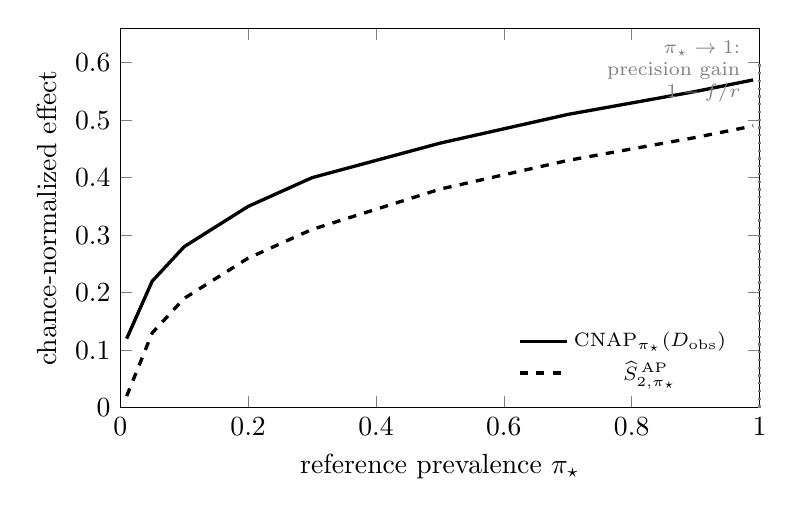
\begin{tikzpicture}
\begin{axis}[
  width=0.80\textwidth, height=6.4cm,
  xlabel={reference prevalence $\pi_\star$},
  ylabel={chance-normalized effect},
  xmin=0, xmax=1.0,
  ymin=0, ymax=0.66,
  xtick={0,0.2,0.4,0.6,0.8,1.0},
  ytick={0,0.1,0.2,0.3,0.4,0.5,0.6},
  legend pos=south east,
  legend style={font=\scriptsize, draw=none, fill=none},
  every axis plot/.append style={very thick},
  clip=false,
]
\addplot[black, mark=none] coordinates {
 (0.01,0.12) (0.05,0.22) (0.10,0.28) (0.20,0.35) (0.30,0.40)
 (0.50,0.46) (0.70,0.51) (0.90,0.55) (0.99,0.57)};
\addlegendentry{$\Tpi(D_{\mathrm{obs}})$}
\addplot[black, dashed, mark=none] coordinates {
 (0.01,0.02) (0.05,0.13) (0.10,0.19) (0.20,0.26) (0.30,0.31)
 (0.50,0.38) (0.70,0.43) (0.90,0.47) (0.99,0.49)};
\addlegendentry{$\SAPHat$}
\draw[gray, dotted, thick] (axis cs:1.0,0) -- (axis cs:1.0,0.60);
\node[gray, font=\scriptsize, anchor=north east, align=right]
  at (axis cs:0.985,0.655) {$\pi_\star\to1$:\\ precision gain\\ $1-f/r$};
\end{axis}
\end{tikzpicture}
\caption{Illustrative reference-prevalence profile for one model. Both curves shown are nondecreasing. Equation~\eqref{eq:reference-prevalence-derivative} guarantees threshold-level monotonicity wherever $r_k\geq f_k$; profiles can be nonmonotone when thresholds cross the ROC diagonal. The right-hand edge marks the limit at which the threshold-level integrand coincides with prevalence-free precision gain. Values are illustrative.}
\label{fig:profile}
\end{figure}

\subsection{Empirical definition}

Let
\[
D=\{(s_i,y_i)\}_{i=1}^{n},
\qquad y_i\in\{0,1\},
\]
with $n_+=\sum_i y_i>0$ and $n_-=n-n_+>0$. Let
\[
c_1>c_2>\cdots>c_K
\]
be the distinct observed score values. Threshold $k$ selects every observation with $s_i\geq c_k$. Define
\[
\operatorname{TP}_k
=
\sum_{i=1}^{n}\mathbf{1}\{y_i=1,\ s_i\geq c_k\},
\qquad
\operatorname{FP}_k
=
\sum_{i=1}^{n}\mathbf{1}\{y_i=0,\ s_i\geq c_k\},
\]
and
\[
r_k=\frac{\operatorname{TP}_k}{n_+},
\qquad
f_k=\frac{\operatorname{FP}_k}{n_-}.
\]
Prior-standardized precision at the threshold is
\begin{equation}
p_{\pi_\star,k}
=
\frac{\pi_\star r_k}
{\pi_\star r_k+(1-\pi_\star)f_k}.
\label{eq:empirical-reference-precision}
\end{equation}
Set $r_0=0$. Prior-standardized average precision is
\begin{equation}
\AP_{\pi_\star}(D)
=
\sum_{k=1}^{K}
(r_k-r_{k-1})p_{\pi_\star,k}.
\label{eq:standardized-ap}
\end{equation}
A threshold that adds only negative cases has $r_k-r_{k-1}=0$. Its false positives still affect precision at later thresholds.

Equation~\eqref{eq:standardized-ap} evaluates precision at thresholds determined by the observed positions of positive cases. This is the source of the upward bias $\beta$ in Equation~\eqref{eq:two-distortions}, since those positions are favorably placed by chance more often than the population baseline implies.

\subsection{Equal scores}

Equal scores form one threshold block. Every observation in the block enters the selected set at the same threshold. This rule uses only distinctions made by the model.

Consider the scores and classes
\[
(0.90,+),\quad(0.70,+),\quad(0.70,-),\quad(0.20,-).
\]
An arbitrary ordering of the two middle cases can produce ordinary AP of $1$ or $5/6$. The model assigns them the same score. Under the block rule, both enter at threshold $0.70$. Precision is then $2/3$ and recall rises from $1/2$ to $1$. Equation~\eqref{eq:standardized-ap}, with the observed prevalence used as the reference prevalence, gives
\[
\AP
=
\frac12(1)+\frac12\left(\frac23\right)
=
\frac56.
\]
Use the model's unrounded numerical scores when they are available. Rounding before evaluation can create ties that were absent from the model output. Because the permutation null of Section~\ref{sec:calibration} preserves the score multiset, it also preserves the tie structure, and the resulting chance level reflects the ties actually present.

\subsection{Average-precision convention}

Equation~\eqref{eq:standardized-ap} uses non-interpolated stepwise average precision. Each increase in recall receives the precision at the threshold that produced it.

Trapezoidal PR area joins adjacent operating points with straight lines. Interpolated AP replaces the empirical precision sequence with a precision envelope. These conventions can give different finite-sample values, and they carry different chance levels. All supported-AP calculations in this document use the stepwise convention in Equation~\eqref{eq:standardized-ap}.

\subsection{Equivalent weighted implementation}

The same quantity can be calculated by assigning each observation the class weight
\begin{equation}
w_i
=
\begin{cases}
\pi_\star/n_+, & y_i=1,\\[4pt]
(1-\pi_\star)/n_-, & y_i=0.
\end{cases}
\label{eq:reference-weights}
\end{equation}
The positive weights sum to $\pi_\star$. The negative weights sum to $1-\pi_\star$. At threshold $k$, weighted precision is
\[
\frac{(\pi_\star/n_+)\operatorname{TP}_k}
{(\pi_\star/n_+)\operatorname{TP}_k
+
\{(1-\pi_\star)/n_-\}\operatorname{FP}_k}
=
p_{\pi_\star,k},
\]
and weighted recall is
\[
\frac{(\pi_\star/n_+)\operatorname{TP}_k}{\pi_\star}
=
r_k.
\]
A weighted AP routine therefore returns $\AP_{\pi_\star}(D)$ when it groups equal scores and uses non-interpolated stepwise AP.

Under the canonical stratified bootstrap, $n_+^{(b)}=n_+$ and $n_-^{(b)}=n_-$ for every replicate. Recalculate the threshold counts, $r_k^{(b)}$, and $f_k^{(b)}$ within each replicate while keeping $\pi_\star$ fixed. When the declared regime allows class counts to vary, use the replicate-specific $n_+^{(b)}$ and $n_-^{(b)}$ in the class weights. Each replicate must contain both outcome classes. A procedure that drops zero-class executions changes the regime-relative replication distribution and requires an explicit conditional estimand.

The prevalence transformation holds the class-conditional score mechanism invariant while the class prior moves to $\pi_\star$. Prior-probability shift is exactly that environment change. A change in the composition of either class alters the mechanism assumed invariant and voids the transformation, which is the failure mode of any regime whose declared invariance does not hold.

\section{Properties of the support functional}
\label{app:properties}

\subsection{Common support}

\begin{proposition}
For realized values $t_1$ and $t_2$, the largest real number that does not exceed either value is $\min(t_1,t_2)$.
\end{proposition}

\begin{proof}
Every admissible level $s$ satisfies $s\leq t_1$ and $s\leq t_2$, so $s\leq\min(t_1,t_2)$. The value $\min(t_1,t_2)$ satisfies both inequalities. It is therefore the largest admissible level.
\end{proof}

\subsection{Disagreement decomposition}

\begin{proposition}
If $\Theta_{\pi_\star,1}$ and $\Theta_{\pi_\star,2}$ are independent and identically distributed with finite first moment, then
\[
\E\min(\Theta_{\pi_\star,1},\Theta_{\pi_\star,2})
=
\E\Theta_{\pi_\star}
-
\frac12
\E|\Theta_{\pi_\star,1}-\Theta_{\pi_\star,2}|.
\]
\end{proposition}

\begin{proof}
Use
\[
\min(a,b)=\frac{a+b-|a-b|}{2}
\]
and take expectations. Identical distributions give
\[
\E\Theta_{\pi_\star,1}
=
\E\Theta_{\pi_\star,2}
=
\E\Theta_{\pi_\star}.
\]
\end{proof}

\subsection{Quantile representation}

Let $Q_{\pi_\star}(u)$ be a generalized quantile function of $\Theta_{\pi_\star}$. If $\E|\Theta_{\pi_\star}|<\infty$, then
\begin{equation}
S_K
=
\int_0^1 K(1-u)^{K-1}Q_{\pi_\star}(u)\,du,
\qquad
\SAP
=
\int_0^1 2(1-u)Q_{\pi_\star}(u)\,du.
\label{eq:quantile}
\end{equation}

To see this, write $\Theta_{\pi_\star,i}=Q_{\pi_\star}(U_i)$ for independent $U_i\sim\operatorname{Uniform}(0,1)$. Since $Q_{\pi_\star}$ is nondecreasing,
\[
\min_i\{Q_{\pi_\star}(U_i)\}
=
Q_{\pi_\star}\{\min_i(U_i)\}.
\]
The minimum of $K$ independent uniform variables has density $K(1-u)^{K-1}$ on $(0,1)$.

Ordinary expectation weights quantiles uniformly. Equation~\eqref{eq:quantile} gives greater weight to lower quantiles through the $K$-replication criterion, and the weighting becomes more concentrated on the lower tail as $K$ increases.

\subsection{Two established families}
\label{app:families}

The operator coincides with objects defined elsewhere, and the identification supplies several properties without separate proof.

\paragraph{L-moments.}
The first two L-moments of a distribution~\cite{hosking1990lmoments} are $\lambda_1=\E[T]$ and $\lambda_2=\tfrac12\E|T_1-T_2|$, the latter being half the Gini mean difference. Equation~\eqref{eq:general-decomposition} is therefore the exact identity
\[
S_2(T;\Regime)=\lambda_1-\lambda_2 .
\]
L-moment estimators are linear in order statistics, which is the origin of the sorted-sum form in Appendix~\ref{app:computation}, and they exist whenever the first moment does.

\paragraph{Distortion risk measures.}
Equation~\eqref{eq:quantile} expresses $S_K$ as a distortion measure with distortion function $g(u)=1-(1-u)^{K}$, a member of the dual-power family in the sense of Wang~\cite{wang1996premium}. Because $g$ is concave, the following hold immediately: monotonicity with respect to first-order stochastic dominance; monotonicity with respect to the concave order, so that a mean-preserving spread of the replication distribution cannot raise $S_2$; translation equivariance, $S_2(T+c)=S_2(T)+c$; positive homogeneity, $S_2(aT)=aS_2(T)$ for $a>0$; comonotone additivity; superadditivity on gains, $S_2(X+Y)\geq S_2(X)+S_2(Y)$, with equality exactly when $X$ and $Y$ are comonotone; and concavity as a functional of the gain variable. The first is proved directly below. Section~\ref{sec:support} uses the concave-order property, and Section~\ref{sec:paired} uses the superadditivity.

\paragraph{Selection by the replication-survival criterion.}
A claim retained by $K$ replications cannot exceed any of their realized effects, so their minimum is the greatest retained level. Averaging this level over the regime gives $S_K$. The replication-survival criterion determines the operator. Its distortion representation places the resulting functional in the dual-power family and supplies the properties above.

\paragraph{U-statistics.}
Equation~\eqref{eq:uestimator} is a U-statistic of degree two with kernel $h(t_i,t_j)=\min(t_i,t_j)$, so its behavior as $B$ grows follows from the theory of Hoeffding~\cite{hoeffding1948ustat}, with variance governed by the projection $h_1(t)=\E[\min(t,T)]$. This concerns Monte Carlo accuracy for fixed $\PRepHat$ and not the statistical information in $D_{\mathrm{obs}}$.

\subsection{Perfect separation under the canonical bootstrap}
\label{app:fixed-point-proof}

\begin{proof}[Proof of Proposition~\ref{prop:fixed-point}]
Stratified resampling draws positive units from $D_{\mathrm{obs},+}$ and negative units from $D_{\mathrm{obs},-}$, so every positive score in each replicate exceeds every negative score. The first threshold block containing a positive unit therefore has $f_k=0$, giving $p_{\pi_\star,k}=1$ whenever recall increases. Thus $\AP_{\pi_\star}(D^{(b)})=1$ and $t_b=1$ in every replicate. The replication distribution is degenerate, so the minimum of two independent draws equals one almost surely.
\end{proof}

\subsection{Affine equivariance}
\label{app:affine-equivariance}

For $a>0$ and constant $c$,
\[
\min(aT_1+c,aT_2+c)
=
a\min(T_1,T_2)+c.
\]
Taking expectations gives
\[
S_2(aT+c;\Regime)=aS_2(T;\Regime)+c.
\]
Chance normalization can therefore be applied before or after the support operator with the same result.

\subsection{Equal summaries with different lower tails}
\label{app:collision-tail}

The mean and disagreement penalty do not determine the full replication distribution. For an equiprobable three-point distribution, the penalty depends only on the range, so the support can move while its range and sum remain fixed.

\begin{table}[ht]
\centering
\caption{Two replication distributions agreeing on the whole of Equation~\eqref{eq:decomposition} and differing in the lower tail.}
\label{tab:collision-tail}
\begin{tabular}{@{}lcccc@{}}
\toprule
Equiprobable support & $\E[\Theta_{\pi_\star}]$ & penalty & $\SAP$ & $m_{0.5}$ \\
\midrule
$\{0.0,\,0.6,\,0.6\}$ & $0.400$ & $0.133$ & $0.267$ & $0.00$ \\
$\{0.2,\,0.2,\,0.8\}$ & $0.400$ & $0.133$ & $0.267$ & $0.20$ \\
\bottomrule
\end{tabular}
\end{table}

The first distribution fails outright in one replication out of three. The second never falls below $0.2$. Their different values of $m_{0.5}$ expose a lower-tail distinction that the common mean, penalty, and supported value do not.

\subsection{Why marginal support values overstate paired support}
\label{app:marginal-proof}

\begin{proof}[Proof of the marginal-superiority proposition]
Equation~\eqref{eq:quantile} represents $S_2$ as a distortion measure with concave distortion $g(u)=1-(1-u)^2$. A concave distortion is superadditive on gains,
\[
S_2(X+Y)\geq S_2(X)+S_2(Y),
\]
with equality exactly when $X$ and $Y$ are comonotone. Apply this result to
\[
\CNAP_{A,\pi_\star}
=
\CNAP_{B,\pi_\star}+\Delta_{\pi_\star}
\]
and rearrange.
\end{proof}

For a numerical example, consider two equally likely evaluation contexts:
\begin{center}
\begin{tabular}{@{}lccc@{}}
\toprule
Context & $\CNAP_{A,\pi_\star}$ & $\CNAP_{B,\pi_\star}$ & $\Delta_{\pi_\star}$ \\
\midrule
1 & $0.90$ & $0.80$ & $0.10$ \\
2 & $0.40$ & $0.10$ & $0.30$ \\
\bottomrule
\end{tabular}
\end{center}
The paired difference takes values $0.10$ and $0.30$, giving
\[
S_2(\Delta_{\pi_\star};\Regime)=0.15.
\]
The marginal support values are
\[
S_2(\CNAP_{A,\pi_\star};\Regime)=0.525,
\qquad
S_2(\CNAP_{B,\pi_\star};\Regime)=0.275,
\]
so their difference is $0.25$. Model $A$ has its largest advantage where model $B$ performs worst, producing the gap between the marginal and paired quantities.

\subsection{Conservatism and consistency}

The inequality
\[
\min(\Theta_{\pi_\star,1},\Theta_{\pi_\star,2})
\leq
\frac{\Theta_{\pi_\star,1}+\Theta_{\pi_\star,2}}{2}
\]
gives $\SAP\leq\E\Theta_{\pi_\star}$.

Suppose $\Theta_{\pi_\star,n}\to t_0$ in probability and all $\Theta_{\pi_\star,n}$ lie in a common bounded interval. Then two independent copies satisfy
\[
\min(\Theta_{\pi_\star,n,1},\Theta_{\pi_\star,n,2})\to t_0
\]
in probability. Bounded convergence gives
\[
\E\min(\Theta_{\pi_\star,n,1},\Theta_{\pi_\star,n,2})\to t_0.
\]
If the corresponding conditional permutation level converges to zero, Equation~\eqref{eq:calibrated} converges to $t_0$.

\subsection{Monotonicity}

Let $Q_A$ and $Q_B$ be quantile functions with $Q_A(u)\geq Q_B(u)$ for all $u\in(0,1)$. Equation~\eqref{eq:quantile} gives
\[
S_2(A)\geq S_2(B).
\]
This condition is first-order stochastic dominance.

\subsection{Centering}
\label{app:centering}

The primary definition is replication-centered:
\[
S_{\mathrm{rep}}
=
\E_{\mathrm{rep}}
\left[
\min(\Theta_{\pi_\star,1},\Theta_{\pi_\star,2})
\right].
\]
It includes the location of expected performance across replications and the disagreement between replications.

A data-centered alternative is
\[
S_{\mathrm{obs}}
=
\Tpi(D_{\mathrm{obs}})
-
\frac12
\E_{\PRepHat}
\left[
|\Theta_{\pi_\star,1}-\Theta_{\pi_\star,2}|
\mid D_{\mathrm{obs}}
\right].
\]
It preserves the observed point estimate and subtracts the estimated disagreement penalty. The replication-centered form is preferred because it matches the target of expected performance across replications and because it is a functional of a single declared distribution, whereas the data-centered form mixes a realized value with a resampling summary. Simulation should compare both forms under finite samples and model misspecification.

\section{Efficient computation}
\label{app:computation}

Let $t_1,\ldots,t_B$ be independent draws from the distribution whose support functional is being calculated, usually $\PRepHat(\cdot\mid D_{\mathrm{obs}})$. Sort them so that
\[
t_{(1)}\leq t_{(2)}\leq\cdots\leq t_{(B)}.
\]
The value $t_{(i)}$ is the minimum in each pair formed with one of the $B-i$ larger values. Equation~\eqref{eq:uestimator} becomes
\begin{equation}
\SAPHatB
=
\frac{2}{B(B-1)}
\sum_{i=1}^{B-1}(B-i)t_{(i)}.
\label{eq:sorted}
\end{equation}

Sorting followed by one weighted sum gives the whole calculation, at cost $O(B\log B)$.

For general $K$, the same argument gives
\[
\widehat S_{K,B}
=
\binom{B}{K}^{-1}
\sum_{i=1}^{B-K+1}
\binom{B-i}{K-1}
t_{(i)},
\]
since $t_{(i)}$ is the minimum of exactly $\binom{B-i}{K-1}$ subsets of size $K$.

\subsection{Monte Carlo standard error}
\label{app:mcse}

The leading Monte Carlo variance of the degree-two U-statistic is governed by the Hoeffding projection $h_1(t)=\E[\min(t,\Theta_{\pi_\star})]$. A leave-one-out estimate on the sorted replicate array is
\begin{equation}
\widehat h_{1,-i}(t_{(i)})
=
\frac{1}{B-1}
\left\{
\sum_{j<i}t_{(j)}
+
(B-i)\,t_{(i)}
\right\},
\qquad
\widehat{\operatorname{se}}_{\mathrm{MC}}
=
\frac{2}{\sqrt{B}}
\operatorname{sd}_{1\leq i\leq B}
\{\widehat h_{1,-i}(t_{(i)})\}.
\label{eq:mcse}
\end{equation}
This is a first-order standard error. Finite-$B$ corrections are of smaller order. One prefix sum over the already sorted array supplies the calculation.

\subsection{Empirical survival levels}
\label{app:survival-computation}

For $K=2$, the empirical frequency-qualified retained level is
\[
\widehat m_\gamma
=
t_{\left(\max\{1,\lceil B(1-\sqrt{\gamma})\rceil\}\right)}.
\]
It is one index into the sorted replication array. For general $K$, replace $1-\sqrt{\gamma}$ by $1-\gamma^{1/K}$.

\subsection{Cost of conditional-null calibration}

The calibrated score repeats this once per permutation, so sorting contributes $O(MB\log B)$ and the $MB$ resampling steps contribute $O(MBn)$, each rebuilding the threshold counts and sweeping them once. The second term dominates whenever $n>\log B$. Permutations are independent jobs and run in parallel, and a stable location estimate needs fewer of them than a small $p$-value.

\section{Conditional-null examples and reporting}

\subsection{Finite-design null examples}
\label{app:null-examples}

The smallest example makes the upward finite-sample AP bias visible. Take $n=2$ with one positive and $\pi_\star=\tfrac12$. If the positive ranks first, $\AP=1$; if second, $\AP=\tfrac12$. Hence $\E[\AP]=0.75$ against a population baseline of $0.5$, and $\E[\Tpi]=0.5$ despite the population value of zero.

For a less extreme case, take $n=10$ with $n_+=1$ and $\pi_\star=\pi=0.1$ under random ranking. The positive occupies rank $j$ with probability $1/10$, and AP with one positive is $1/j$. Therefore
\[
\E[\AP]=\frac{H_{10}}{10}=0.2929,
\qquad
\beta=\E[\Tpi]=\frac{H_{10}-1}{9}=0.2143,
\]
where $H_n=\sum_{j=1}^n1/j$. The disagreement penalty is
\[
\delta
=
\frac12\E\left|\Theta_{\pi_\star,1}-\Theta_{\pi_\star,2}\right|
=
0.1358.
\]
Their difference gives the finite-design supported chance level,
\begin{equation}
S_2(\CNAP_{\pi_\star};\Regime_0)
=
\frac{10-H_{10}}{90}
=
0.0786.
\label{eq:worked-null}
\end{equation}
For general $n$ with $n_+=1$ and $\pi_\star=1/n$,
\[
\beta=\frac{H_n-1}{n-1},
\qquad
S_2(\CNAP_{\pi_\star};\Regime_0)
=
\frac{n-H_n}{n(n-1)}.
\]

\subsection{Complete reporting example}
\label{app:report-example}

A report states the reference prevalence, observed and replication counts, regime, resampling and permutation methods, exchangeable units, computational counts, Monte Carlo stability, and separation of prediction development from evaluation outcomes. For example:
\begin{quote}
At a reference prevalence of $0.10$, conditionally calibrated supported AP was $0.247$. Supported chance-normalized AP, $\widehat S_{2,0.10}^{\,\mathrm{AP}}$, was $0.270$, and mean chance-normalized AP across empirical replications was $0.298$, giving a disagreement penalty of $0.028$. The conditional permutation null was $0.031$, with $p<0.002$. The calibrated scale assigns this conditional chance level zero and perfect separation one. The observed chance-normalized AP, $\CNAP_{0.10}(D_{\mathrm{obs}})$, was $0.340$. The held-out evaluation contained 100 positive and 900 negative patients. Each of $5{,}000$ stratified bootstrap replicates sampled 100 positive and 900 negative patients with replacement from their observed classes. The null held the score vector fixed and used $500$ outcome permutations across patients, each followed by the same $5{,}000$-replicate procedure. Doubling $B$ and $M$ left both supported estimates stable to three decimal places.
\end{quote}

\section{Additional Bank Marketing diagnostics}
\label{app:bank-diagnostics}

\subsection{Design-specific chance levels}

The conditional-null grid holds real logistic-regression scores fixed, permutes labels, and varies positive count and score resolution. Rows vary the positive count from 5 to 100 while maintaining prevalence near $\pi_\star$. Columns quantize the scores to 2, 5, or 20 levels or retain their continuous values.

\begin{figure}[htbp]
\centering
\includegraphics[width=\textwidth]{manuscript_images/03-design-specific-chance.pdf}
\caption{Conditional-null supported chance-normalized AP for the full logistic model. Real held-out scores were quantized to the stated number of levels, and labels were permuted within samples with the stated positive counts. Every cell is $\SAPnullHat$ from $B=1{,}200$ bootstrap replications within each of $M=100$ outcome permutations. The reference prevalence is $\pi_\star=0.06373$.}
\label{fig:bank-conditional-null}
\end{figure}

\subsection{Calibration under permuted outcomes}

The calibration diagnostic applies the design-specific transformation to 160 independently permuted label vectors under four real-score designs. Each permuted dataset generates its own empirical replication distribution and estimated null anchor, so individual calibrated values still vary even when their mean is near zero.

\begin{figure}[htbp]
\centering
\includegraphics[width=\textwidth]{manuscript_images/04-calibration-restores-zero.pdf}
\caption{Conditional-null calibration under four held-out score designs from the full logistic model. Each violin contains the values obtained from 160 label permutations. Panel A reports raw $\SAPHat$ under permuted labels. Panel B reports $\SAPcalHat$ after the conditional-null anchor for that evaluation is assigned zero and perfect separation is assigned one. Whiskers give the mean plus or minus 1.96 standard errors across the 160 permutations. Each value uses $B=600$ bootstrap replications and $M=60$ inner permutations.}
\label{fig:bank-calibration}
\end{figure}

\subsection{Sparse positive outcomes}

Eighteen held-out samples were drawn at each positive count from 5 to 100 at prevalence near $\pi_\star$. The figure shows both the reporting sequence and the total observed-to-calibrated adjustment.

\begin{figure}[htbp]
\centering
\includegraphics[width=\textwidth]{manuscript_images/05-real-data-sparse-outcomes.pdf}
\caption{The practical size of the complete adjustment for the full logistic model. Panel A shows the median reporting sequence $\Tpi(D_{\mathrm{obs}})\rightarrow\SAPHat\rightarrow\SAPcalHat$ at five and 100 positive outcomes. Panel B reports the median paired difference $\Tpi(D_{\mathrm{obs}})-\SAPcalHat$ across all positive counts; the band spans its 10th to 90th percentiles over 18 real held-out samples. Every supported value uses $B=600$ bootstrap replications, and every calibrated value uses $M=60$ permutations.}
\label{fig:bank-sparse}
\end{figure}

\subsection{Same-design model-superiority profile}

The final diagnostic changes both the observed counts and the replication counts inherited by the canonical bootstrap. It therefore compares different same-design corroboration questions rather than the estimation of one fixed prospective target.

\begin{figure}[htbp]
\centering
\includegraphics[width=\textwidth]{manuscript_images/07-evidence-for-model-superiority.pdf}
\caption{Observed and supported random-forest superiority across same-design evaluations. Each row changes both the observed counts and the replication counts inherited by the canonical bootstrap. The models remain fixed. Circles mark median $\Delta_{\pi_\star}(D_{\mathrm{obs}})$, squares mark median $\widehat S_{2,B}(\Delta_{\pi_\star};\Regime)$, and arrows show their adjustment. Thin intervals span the 10th to 90th percentiles over 12 held-out subsamples. Subsamples use $B=500$ paired replications; the full holdout uses $B=3{,}000$.}
\label{fig:bank-superiority-information}
\end{figure}

\end{document}
